% Appendices to the manuscript, merged into the single document TMLR expects.
% Until 2026-09-08 these were a separate supplementary PDF, because Pattern Recognition
% counts appendices against a 35-page limit; TMLR does not, so they are back inline and
% every cross-reference is a plain \ref again.

\section{A worked example}\label{app:worked}

Four data points are enough to show the whole construction, and to exhibit in arithmetic
the main properties Section~\ref{sec:method} proves in general. Take one cell containing
four test cases and two possible labels. Three of the cases carry label $1$ and one
carries label $2$, so the cell's label frequencies are $(3/4,1/4)$. The old model $q_0$
is uninformative within the cell: it predicts $(0.5,0.5)$ for all four cases. We compare
two candidate replacements, shown in Table~\ref{tab:worked}.

\begin{table}[t]
\centering
\small
\caption{A four-point example in a single cell. Model A moves every case to the cell's
label frequencies; model B moves each case towards its own correct label by the same
amount. The two models are equally far from $q_0$, and only B uses information about the
individual case.}
\label{tab:worked}
\begin{tabular}{@{}ccccc@{}}
\toprule
case $i$ & label $y_i$ & $q_0(\cdot\mid x_i)$ & model A: $q_1(\cdot\mid x_i)$ &
model B: $q_1(\cdot\mid x_i)$ \\
\midrule
1 & 1 & $(0.5,0.5)$ & $(0.75,0.25)$ & $(0.75,0.25)$ \\
2 & 1 & $(0.5,0.5)$ & $(0.75,0.25)$ & $(0.75,0.25)$ \\
3 & 1 & $(0.5,0.5)$ & $(0.75,0.25)$ & $(0.75,0.25)$ \\
4 & 2 & $(0.5,0.5)$ & $(0.75,0.25)$ & $(0.25,0.75)$ \\
\bottomrule
\end{tabular}
\end{table}

Score both models with the quadratic score $S(q,y)=2q_y-\lVert q\rVert_2^2$, and for each
case tabulate the score \emph{difference} at each of the two possible labels, not only at
the observed one. Writing $h_i(y)=S(q_1(\cdot\mid x_i),y)-S(q_0(\cdot\mid x_i),y)$, all
the arithmetic is in eighths:
\begin{equation}
h_i(y)=
\begin{cases}
+3/8 & \text{if $y$ is the label the new model moved towards},\\
-5/8 & \text{otherwise}.
\end{cases}
\label{eq:worked-h}
\end{equation}
This vector, evaluable at labels that were never observed for case $i$, is the only object
the method needs beyond the labels themselves.

\paragraph{Model A: a pure prior refit.}
Every case gets the same prediction, so $h_i(1)=+3/8$ and $h_i(2)=-5/8$ throughout, and the
observed mean gain is $\Delta T=\tfrac14[3\cdot\tfrac38-\tfrac58]=\tfrac18$. Now transport:
replace each case's label in turn by each of the other three and average. Cases 1--3 are
each scored against $\{1,1,2\}$, giving $\tfrac13(\tfrac38+\tfrac38-\tfrac58)=\tfrac1{24}$;
case 4 is scored against $\{1,1,1\}$, giving $+\tfrac38$. So
$\Delta P=\tfrac14[3\cdot\tfrac1{24}+\tfrac38]=\tfrac18$ and $\Delta R=0$ --- exactly, in
this sample, not on average over hypothetical resamples. That is the general fact: a
prediction change constant within a cell contributes nothing to $\Delta R$
(Theorem~\ref{thm:population}). Note also that $\Delta P=1/8$ is the largest transported
gain any within-cell-constant prediction can earn here, since a proper score is maximised in
expectation at the true frequencies $(3/4,1/4)$ --- which is what A predicts.

\paragraph{Model B: a case-specific improvement.}
Cases 1--3 are unchanged, but case 4 now moves towards label $2$, so $h_4(1)=-5/8$ and
$h_4(2)=+3/8$. Every case is scored at $+3/8$ on its own label, so $\Delta T=3/8$. Under
transport cases 1--3 are unaffected, but case 4 is scored against three label-1 cases at
$-5/8$ apiece, so $\Delta P=\tfrac14[3\cdot\tfrac1{24}-\tfrac58]=-\tfrac18$ and
$\Delta R=\tfrac12$.

Two things follow. First, B's aggregate gain of $3/8$ \emph{understates} its case-level
improvement of $1/2$, and not because B fits the cell frequencies worse --- it fits them
better, moving the cell-mean prediction from $0.5$ to $0.625$ against a truth of $0.75$, an
improvement of exactly $0.09375$. What offsets it is dispersion: B's forecasts vary inside
the cell where the old model's did not, and by Proposition~\ref{prop:transported} the
transported channel charges that variation at the same $0.09375$, so the two cancel and the
in-sample transported gain is zero. The $-1/8$ the estimator reports is what remains once
each case is scored against the \emph{other} cases' labels only, removing the
$\tfrac1{n_c}\widehat{\Delta R}=1/8$ the in-sample plug-in had credited to the transported
channel. Second, an evaluator reading only the total would credit B with three times A's
improvement, whereas the two improve on disjoint grounds: A earns $1/8$ purely by moving to
the cell frequencies and gains no covariance, while B's $1/2$ of covariance is partly
concealed by a transported term that turns negative. This is the failure mode that motivates
the paper, in miniature --- aggregate scores are not merely imprecise about composition, they
can order two models by the wrong criterion.

\paragraph{The covariance form, and why leaving one out matters.}
Theorem~\ref{thm:population} says $\Delta R$ is a within-cell covariance between the
probability change and the label indicator. Computing it directly for model B gives
$2\sum_y\operatorname{Cov}(\Delta q_y,\ind\{Y=y\})=3/8$, not the $1/2$ transport returned.
Neither is wrong: the covariance uses the cell's \emph{own} four labels to form its
reference, so each case contributes to the reference it is compared against, and that
in-sample plug-in is attenuated by exactly $(n_c-1)/n_c=3/4$ --- indeed
$\tfrac34\cdot\tfrac12=\tfrac38$. Transport, which scores each case only against the
\emph{other} cases' labels, removes the attenuation with no held-out data.
Proposition~\ref{prop:attenuate} shows this holds for every cell with $n_c\ge2$ and every
grouping variable, which is why the method needs no sample splitting. The example is
reproduced as a unit test in the accompanying software.

One property the example cannot show, because both candidates happen to be equally
confident, is the estimator's sensitivity to confidence itself. Multiply every prediction's
odds by a constant and $\Delta R$ moves, though no case has been reordered and no
information added; Section~\ref{sec:simulation} measures that at $-0.488$ in a design where
the two models carry identical case-level information. Every result in this paper is
therefore reported for confidence-matched pairs.

\paragraph{A decision the split changes.}\label{sec:decision}
At the benchmark's own label frequencies both candidates improve and B improves three times
as much, so an evaluator reading the score picks B, rightly. Suppose deployment sees label
frequencies in this cell of $(\tfrac14,\tfrac34)$ instead of the observed
$(\tfrac34,\tfrac14)$ --- a label shift, the situation post-hoc prior correction addresses
\citep{saerens2002adjusting,lipton2018detecting}. Reweighting each case by $p'(y_i)/p(y_i)$
and rescoring sends A from $+\tfrac18$ to $-\tfrac38$ while leaving B at $+\tfrac38$: A
becomes \emph{worse} than the model it was meant to replace, on a change that leaves every
prediction exactly as it was. The decomposition says in advance which is exposed and the
aggregate score does not, because A's whole gain sits in the transported channel --- the one
a change in label frequencies acts on --- and B's in the covariance channel, which such a
change leaves alone. That is the operational content of the split: $\widehat{\Delta P}$ is
the part of a reported improvement contingent on the evaluation set's label frequencies
matching deployment, and $\widehat{\Delta R}$ is the part that is not.
Section~\ref{sec:vgvisual} exhibits the same structure on real models.

\begin{figure*}[t]
\centering
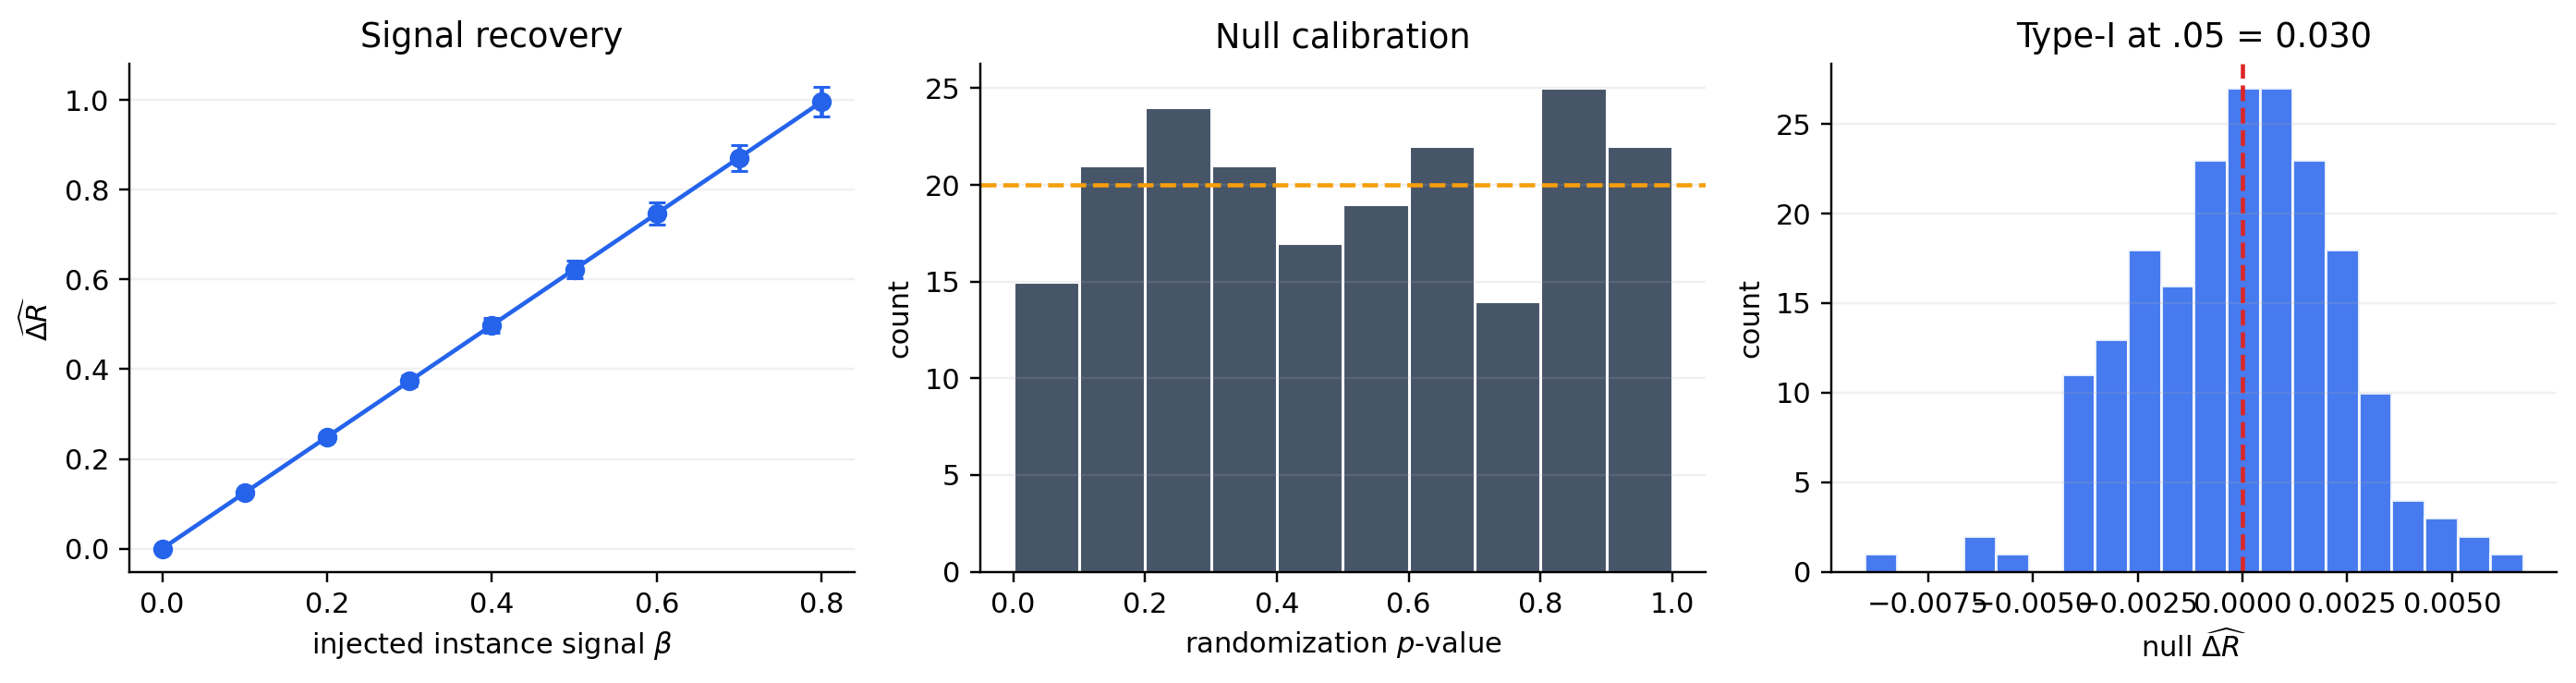
\includegraphics[width=\textwidth]{figures/fig3_new_simulation.png}
\caption{\textbf{Controlled validation.} WAGER recovers injected within-cell signal
monotonically (mean $\pm$ one standard deviation), produces approximately uniform null
randomization $p$-values, and controls type-I error in 200 null runs.}
\label{fig:simulation}
\end{figure*}

\section{Coarsening and unrecorded covariates}\label{app:coarsen}

Appendix~\ref{sec:ablations} reports that replacing the class-pair cell with a coarser
subject-only cell changes the estimated covariance gain. The following result gives that
sensitivity an exact population-level mechanism rather than treating it as an empirical
curiosity.


The first term is the coarse cell's share of the fine-grained covariance gain; the second is
a between-cell covariance, over the finer cells nested inside $\bar c$, between each fine
cell's typical gain at label $y$ and its label-$y$ frequency. It is not sign definite, so
coarsening $\phi$ can inflate or deflate the credited covariance gain, and it vanishes
exactly when either quantity is constant within each coarse cell. This is why the finest
defensible $\phi$ is the conservative default: coarsening adds cross-cell prior structure
into $\Delta R$, while the finer partition's gain is preserved on average through the first
term. The proof is a per-label application of the law of total covariance
(Appendix~\ref{app:proofs}).

\subsection{Sensitivity to an unrecorded confounder}\label{sec:sensitivity}

Read in one direction, Proposition~\ref{prop:coarsen} says what folding a covariate into
$\phi$ does. Read in the other, it quantifies what happens when a relevant covariate is
\emph{never} declared, which is the estimator's main scope limit. Let $Z$ be unrecorded and
let $(\phi,Z)$ be the finer, fully adjusted cell. Applying
Proposition~\ref{prop:coarsen} with $\bar\phi=\phi$ gives, for every declared cell $c$,
\begin{equation}
\Delta R_c(\phi)=\mathbb E\!\left[\Delta R_{(\phi,Z)}\mid\phi=c\right]
+\sum_{y=1}^K\operatorname{Cov}\!\left(\mathbb E[H_X(y)\mid\phi,Z],\,
\Pr(Y=y\mid\phi,Z)\ \middle|\ \phi=c\right),
\label{eq:sensitivity-exact}
\end{equation}
whose first term is what an analyst who could observe $Z$ would report and whose second is
the bias of using $\phi$ alone. The identity is exact but needs $Z$'s joint law with
$(H,Y)$. The following bound replaces that with a judgement about how strongly an unrecorded
variable could plausibly act, in the spirit of \citet{rosenbaum2002observational}.

Proposition~\ref{prop:sensitivity} states that bound and Corollary~\ref{cor:sensitivity-crude}
its data-free form; both are proved in Appendix~\ref{app:proofs}. Because $\bar\rho$ is a
correlation rather than a domain-specific odds ratio, it can be elicited the same way across
benchmarks. Appendix~\ref{app:sensitivity} evaluates both forms on our own estimates, and
the sharp one is the less comfortable: an unrecorded covariate correlated at $0.061$ would
account for the entire covariance gain reported in Appendix~\ref{sec:results}.



\section{Proofs}\label{app:proofs}

\subsection{Proof of Theorem~\ref{thm:population}}
Condition throughout on $C=c$. Expanding over labels gives
\[
\Delta T_c=\sum_y\mathbb E[H_X(y)\ind \{Y=y\}],\qquad
\Delta P_c=\sum_y\mathbb E[H_X(y)]\Pr(Y=y).
\]
Subtracting yields the covariance sum in Eq.~\eqref{eq:population-id}; the first
identity is the definition of $\Delta R_c$. Under the quadratic score,
\[
H_X(y)=2\Delta q_y(X)-\{\lVert q_1(\cdot\mid X)\rVert_2^2-
\lVert q_0(\cdot\mid X)\rVert_2^2\}.
\]
The bracketed term is independent of the label index. Its contribution summed over $y$
is $\operatorname{Cov}(B(X),\sum_y\ind \{Y=y\})=
\operatorname{Cov}(B(X),1)=0$. The remaining terms give Eq.~\eqref{eq:cov-id}. If
$H_X(y)=H_c(y)$ almost surely, every covariance is zero. \qed

\subsection{Proof of Proposition~\ref{prop:transported}}
Condition on $C=c$ and let $Y'\sim p(c)$ be independent of $X$. For the quadratic score
$S_{\rm B}(q,y)=2q_y-\lVert q\rVert^2$,
\begin{equation}
\mathbb E\bigl[S_{\rm B}(q_m,Y')\mid c\bigr]
=2\bigl\langle p(c),\bar q_m(c)\bigr\rangle-\mathbb E\bigl[\lVert q_m\rVert^2\mid c\bigr].
\end{equation}
Decompose the second moment as
$\mathbb E[\lVert q_m\rVert^2\mid c]=\lVert\bar q_m(c)\rVert^2
+\operatorname{tr}\operatorname{Var}(q_m\mid c)$, and complete the square using
$2\langle p,\bar q\rangle-\lVert\bar q\rVert^2=\lVert p\rVert^2-\lVert p-\bar q\rVert^2$:
\begin{equation}
\mathbb E\bigl[S_{\rm B}(q_m,Y')\mid c\bigr]
=\lVert p(c)\rVert^2-\lVert p(c)-\bar q_m(c)\rVert^2
-\operatorname{tr}\operatorname{Var}(q_m\mid c).
\end{equation}
Subtracting the $m=0$ expression from the $m=1$ expression, the $\lVert p(c)\rVert^2$
terms cancel and Eq.~\eqref{eq:transported-composition} follows, since
$\Delta P_c=\mathbb E[S_{\rm B}(q_1,Y')\mid c]-\mathbb E[S_{\rm B}(q_0,Y')\mid c]$ by
definition. \qed

\subsection{Proof of Theorem~\ref{thm:bregman}}
Condition on $C=c$. The proof of Theorem~\ref{thm:population} above establishes
$\Delta R_c=\sum_y\operatorname{Cov}(H_X(y),\ind\{Y=y\}\mid C=c)$ for \emph{any} score
contrast $H$, not only the quadratic one; only the identification of $H_x(y)$ with a
specific functional form is score-dependent. For the Bregman score of
the Bregman score $S_\psi(q,y)=\psi(q)+\langle\nabla\psi(q),e_y-q\rangle$,
\[
H_x(y)=\underbrace{\bigl[\psi(q_1(x))-\psi(q_0(x))\bigr]
-\bigl[\langle\nabla\psi(q_1(x)),q_1(x)\rangle-\langle\nabla\psi(q_0(x)),q_0(x)\rangle\bigr]}_{=:B(x)}
+\;\Delta g_y(x),
\]
writing $q_i(x)$ for $q_i(\cdot\mid x)$, where $B(x)$ collects every term not indexed by
$y$ and $\Delta g_y(x)=\partial_y\psi(q_1(x))-\partial_y\psi(q_0(x))$ is the $y$-indexed
remainder, exactly as in the proof of Theorem~\ref{thm:population} for the quadratic
case. Substituting,
\begin{align*}
\sum_y\operatorname{Cov}(H_X(y),\ind\{Y=y\}\mid c)
&=\operatorname{Cov}\Bigl(B(X),\sum_y\ind\{Y=y\}\ \Big|\ c\Bigr)\\
&\quad+\sum_y\operatorname{Cov}(\Delta g_y(X),\ind\{Y=y\}\mid c).
\end{align*}
The first term is $\operatorname{Cov}(B(X),1\mid c)=0$ since $\sum_y\ind\{Y=y\}=1$
almost surely. The second term is Eq.~\eqref{eq:bregman-cov-id}. \qed

\subsection{Proof of Theorem~\ref{thm:sample}}
Summing the kernel in Eq.~\eqref{eq:kernel} over unordered pairs, every observed term
$H_i(y_i)$ occurs in $n_c-1$ pairs with coefficient $1/2$, while the two crossed terms
together enumerate every ordered pair $H_i(y_j)$, $i\ne j$, with coefficient $1/2$.
Since $\binom{n_c}{2}=n_c(n_c-1)/2$,
\[
\widehat{\Delta R}_c
=\frac1{n_c}\sum_iH_i(y_i)
-\frac1{n_c(n_c-1)}\sum_{i\ne j}H_i(y_j)
=\widehat{\Delta T}_c-\widehat{\Delta P}_c.
\]
This is deterministic. When the cell's examples are i.i.d.\ draws from the cell
population, the average of the symmetric order-two kernel is the standard unbiased
U-statistic for its population expectation \cite{hoeffding1948class}; independence is
used, not merely exchangeability, because $\Delta P_c$ is defined through an independent
label coupling, so $\mathbb E[H_1(Y_2)]=\mathbb E[H_X(Y')]$ requires the two draws to be
independent. \qed

\subsection{Proof of Proposition~\ref{prop:coarsen}}
Fix $y$ and condition throughout on $\bar\phi=\bar c$. The law of total covariance
applied to the pair $(H_X(y),\ind \{Y=y\})$ with the finer conditioning variable $C$
nested inside $\bar c$ gives
\begin{align*}
\operatorname{Cov}\!\left(H_X(y),\ind \{Y=y\}\mid\bar\phi=\bar c\right)
&=\mathbb E\!\left[\operatorname{Cov}(H_X(y),\ind \{Y=y\}\mid C)
   \;\middle|\;\bar\phi=\bar c\right]\\
&\quad+\operatorname{Cov}\!\left(\mathbb E[H_X(y)\mid C],\,
   \Pr(Y=y\mid C)\;\middle|\;\bar\phi=\bar c\right),
\end{align*}
using $\mathbb E[\ind \{Y=y\}\mid C]=\Pr(Y=y\mid C)$. Summing over $y=1,\ldots,K$ and
applying the population identity of Theorem~\ref{thm:population} to the left side (at
$\bar\phi=\bar c$) and to the first term on the right side (at $C=c$, then averaged over
$c$ within $\bar c$) yields Eq.~\eqref{eq:coarsen}. \qed

\subsection{Proof of Proposition~\ref{prop:attenuate}}
Fix a cell $c$ with $n_c\ge2$ and $i\in c$. By definition of the label count,
$\sum_{y=1}^K m_{cy}H_i(y)=\sum_{j\in c}H_i(y_j)=H_i(y_i)+\sum_{j\ne i}H_i(y_j)$, and
Eq.~\eqref{eq:linear} gives $\sum_{j\ne i}H_i(y_j)=(n_c-1)\hat P_i$. Hence
\[
\tilde P_i=\frac1{n_c}\sum_{y}m_{cy}H_i(y)
=\frac{H_i(y_i)+(n_c-1)\hat P_i}{n_c}.
\]
Substituting $H_i(y_i)=\hat P_i+\hat R_i$ gives
$\tilde P_i=\hat P_i+n_c^{-1}\hat R_i$, and $\tilde R_i=H_i(y_i)-\tilde P_i
=\hat R_i-n_c^{-1}\hat R_i=(n_c-1)n_c^{-1}\hat R_i$. Averaging $\tilde R_i$ within cell
$c$ and reweighting by $n_c$ across cells, as in the dataset-level definition of
$\widehat{\Delta Z}$, gives
$\widetilde{\Delta R}=N_*^{-1}\sum_{c}n_c\cdot\frac{n_c-1}{n_c}\widehat{\Delta R}_c
=N_*^{-1}\sum_c(n_c-1)\widehat{\Delta R}_c$. \qed

\subsection{Proof of Proposition~\ref{prop:sensitivity}}
Fix $\phi=c$ throughout and write $a_y=\mathbb E[H_X(y)\mid\phi,Z]$,
$b_y=\Pr(Y=y\mid\phi,Z)$, both random through their dependence on $(\phi,Z)$. Let
$U=(a_y-\mathbb E[a_y\mid c])_{y=1}^K$ and $V=(b_y-\mathbb E[b_y\mid c])_{y=1}^K$ be the
corresponding mean-zero $\mathbb R^K$-valued random vectors conditional on $\phi=c$. The
map $(U,V)\mapsto\mathbb E[\langle U,V\rangle\mid c]=\sum_y\operatorname{Cov}(a_y,b_y\mid c)$
is an inner product on the space of mean-square-integrable $\mathbb R^K$-valued random
variables conditional on $\phi=c$, so by the Cauchy--Schwarz inequality applied to that
inner product,
\[
\Bigl|\sum_{y=1}^K\operatorname{Cov}(a_y,b_y\mid c)\Bigr|
\le\sqrt{\mathbb E[\lVert U\rVert^2\mid c]}\,\sqrt{\mathbb E[\lVert V\rVert^2\mid c]}
=\sqrt{\textstyle\sum_y\operatorname{Var}(a_y\mid c)}\,\sqrt{\textstyle\sum_y\operatorname{Var}(b_y\mid c)}.
\]
By the definition of $\rho$, the left side equals
$|\rho|\sqrt{\sum_y\operatorname{Var}(a_y\mid c)}\sqrt{\sum_y\operatorname{Var}(b_y\mid c)}$
exactly, so this step alone is not yet a bound; two further steps supply one, at two
different levels of conservatism. First, $a_y=\mathbb E[H_X(y)\mid\phi,Z]$ is itself a
conditional expectation of $H_X(y)$ given more information than $\phi=c$ alone, so the
law of total variance gives $\operatorname{Var}(H_X(y)\mid c)=\mathbb
E[\operatorname{Var}(H_X(y)\mid\phi,Z)\mid c]+\operatorname{Var}(a_y\mid c)\ge
\operatorname{Var}(a_y\mid c)$; likewise $b_y=\Pr(Y=y\mid\phi,Z)$ satisfies
$\operatorname{Var}(b_y\mid c)\le\operatorname{Var}(\ind\{Y=y\}\mid c)=p_y(c)(1-p_y(c))$ by
the same argument applied to $\ind\{Y=y\}$ in place of $H_X(y)$. Both bounds hold
termwise, so summing over $y$ and applying the (monotone) square root to each sum
separately gives the observable, per-cell bound
\[
\sqrt{\textstyle\sum_y\operatorname{Var}(a_y\mid c)}\sqrt{\textstyle\sum_y\operatorname{Var}(b_y\mid c)}
\le\sqrt{\textstyle\sum_y\operatorname{Var}(H_X(y)\mid c)}\sqrt{\textstyle\sum_yp_y(c)(1-p_y(c))},
\]
the second inequality of Eq.~\eqref{eq:sensitivity-bound}; this is a bound on a product of
two sums, and does not simplify to a sum of per-label square roots, since Cauchy--Schwarz
runs the other way for that rearrangement. Second, for
Corollary~\ref{cor:sensitivity-crude}, $a_y\in[-M,M]$ as a conditional expectation of a
$[-M,M]$-valued variable, so Popoviciu's inequality gives
$\operatorname{Var}(a_y\mid c)\le M^2$ for every $y$ and hence
$\sum_y\operatorname{Var}(a_y\mid c)\le KM^2$. For the $b_y$ the same argument would give
$\operatorname{Var}(b_y\mid c)\le1/4$ and a total of $K/4$, but that treats the $b_y$ as
$K$ unconstrained quantities in $[0,1]$ when in fact $\sum_yb_y=1$ almost surely. Using
that constraint, $\sum_yb_y^2\le\bigl(\sum_yb_y\bigr)^2=1$ pointwise, while
$\sum_y(\mathbb E b_y)^2\ge K^{-1}\bigl(\sum_y\mathbb E b_y\bigr)^2=1/K$ by
Cauchy--Schwarz, so
\[
\sum_{y=1}^K\operatorname{Var}(b_y\mid c)
=\mathbb E\Bigl[\sum_yb_y^2\Bigr]-\sum_y\bigl(\mathbb E b_y\bigr)^2\le1-\frac1K,
\]
which is Eq.~\eqref{eq:simplex-var} and is strictly smaller than $K/4$ for every $K>2$.
Therefore
\[
\Bigl|\sum_{y=1}^K\operatorname{Cov}(a_y,b_y\mid c)\Bigr|
\le|\rho|\sqrt{KM^2}\sqrt{1-1/K}=|\rho|\,M\sqrt{K-1}.
\]
By Eq.~\eqref{eq:coarsen}, the left side of each display is exactly
$|\Delta R_c(\phi)-\mathbb E[\Delta R_{(\phi,Z)}\mid\phi=c]|$, giving
Eq.~\eqref{eq:sensitivity-bound} and Eq.~\eqref{eq:sensitivity-crude}. \qed

\section{Influence function: estimand and derivation}\label{app:influence}

\paragraph{The estimand under singleton exclusion.} Cells with $n_c=1$ identify no
within-cell counterfactual and are excluded, so the dataset-level statistic targets the
\emph{identified-subpopulation} quantity: writing $\pi_c$ for the cell probabilities,
the target of $\widehat{\Delta R}$ is the $\pi$-weighted mean
$\theta=\sum_c\pi_c\,\Delta R_c/\sum_c\pi_c$ taken over cells that appear with at least
two examples. At finite $N$ the identified set is random; we treat the interval as
conditional on identification and report the identified fraction alongside every
estimate (99.0\% of relations on VG150, 100\% on CIFAR-100-LT), so the gap between the
conditional and full-population targets is bounded by the reported coverage.

\paragraph{Derivation of Eq.~\eqref{eq:influence}.} Fix a cell $c$ and let
$\theta_c=\Delta R_c$ with $g_c(z)=\mathbb E[A(z,Z')\mid Z'\in c]$ the kernel
projection. The classical H\'ajek projection of the order-two U-statistic
$\widehat{\Delta R}_c$ is
\[
\widehat{\Delta R}_c=\theta_c+\frac{2}{n_c}\sum_{i\in c}\bigl(g_c(Z_i)-\theta_c\bigr)
+O_p(n_c^{-1}).
\]
The dataset statistic weights cells by their example counts,
$\widehat{\Delta R}=N_*^{-1}\sum_c n_c\widehat{\Delta R}_c$, and cell membership is
itself random (multinomial over cells), so an example $i$ contributes both through the
within-cell projection and through the between-cell composition term
$\theta_{C_i}-\theta$. Combining the two sources,
\[
\widehat{\Delta R}-\theta
=\frac{1}{N_*}\sum_{i}\Bigl[2\bigl(g_{C_i}(Z_i)-\theta_{C_i}\bigr)
+\bigl(\theta_{C_i}-\theta\bigr)\Bigr]+o_p(N_*^{-1/2}),
\]
where the dataset-level remainder requires one condition beyond the per-cell expansion,
because $C$ per-cell remainders do not aggregate for free. Writing
$C=\#\{c:n_c\ge2\}$ for the number of eligible cells, the weighted sum of the per-cell
degenerate terms is $N_*^{-1}\sum_cn_c\cdot O_p(n_c^{-1})=O_p(C/N_*)$, which is
$o_p(N_*^{-1/2})$ provided
\begin{equation}
C=o\bigl(\sqrt{N_*}\bigr).
\label{eq:cellcount}
\end{equation}
This is what makes the second-order rate $O_p(n_c^{-1})$ rather than $o_p(n_c^{-1/2})$
worth stating: the sharper per-cell rate is what allows a condition on the cell
\emph{count} alone, with no further requirement on individual cell sizes. On VG150,
$C=6{,}346$ against $N_*=227{,}337$, so $C/\sqrt{N_*}\approx13.3$ --- the condition is a
statement about the limit, and at these finite sample sizes it is the coverage simulation
of Section~\ref{sec:simulation}, not Eq.~\eqref{eq:cellcount}, that supports the reported
intervals.
Estimating $g_{C_i}(Z_i)$ by the pair-kernel mean $\bar A_i$, $\theta_c$ by
$\widehat{\Delta R}_c$, and $\theta$ by $\widehat{\Delta R}$ gives the plug-in
influence contribution
$\widehat\psi_i=2(\bar A_i-\widehat{\Delta R}_{c})+(\widehat{\Delta R}_{c}
-\widehat{\Delta R})=2\bar A_i-\widehat{\Delta R}_{c}-\widehat{\Delta R}$, which is
Eq.~\eqref{eq:influence} and has exactly zero sample mean by construction. Its empirical
95\% coverage in a VG-like regime (image-clustered examples, heavy-tailed cell sizes with
a large mass of near-minimum cells) is validated in Section~\ref{sec:simulation}.

\paragraph{Proof of Theorem~\ref{thm:clt}.} The linearization above gives
$\widehat{\Delta R}-\theta=N_*^{-1}\sum_i\psi_i+o_p(N_*^{-1/2})$, under
Eq.~\eqref{eq:cellcount}, for the population
influence contribution $\psi_i=2(g_{C_i}(Z_i)-\theta_{C_i})+(\theta_{C_i}-\theta)$, which
has zero mean by construction and satisfies $|\psi_i|\le C(M)$ for an absolute constant
$C(M)$ depending only on the score bound $M$ in condition (i), since $g_{C_i}$,
$\theta_{C_i}$, and $\theta$ are themselves averages of the bounded kernel
$A_{ij}\in[-2M,2M]$. Because clusters are mutually independent (condition (ii)),
$T_g=\sum_{i\in g}\psi_i$ for $g=1,\dots,G$ are independent, mean-zero random variables
with $|T_g|\le|g|\,C(M)$. Condition (ii)'s finite third moment for cluster sizes and
$\max_g|g|=o(\sqrt G)$ give
$\sum_gE|T_g|^3\le C(M)^3\sum_g\mathbb E|g|^3=O(G)$ while
$\bigl(\sum_g\operatorname{Var}(T_g)\bigr)^{3/2}=\Theta(G^{3/2})$ under condition (iv), so
Lyapunov's ratio $\sum_gE|T_g|^3/(\sum_g\operatorname{Var}(T_g))^{3/2}\to0$; the
Lyapunov condition implies the Lindeberg condition, and the Lindeberg--Feller central
limit theorem for triangular arrays of independent summands
\citep{serfling1980approximation,vandervaart1998asymptotic} gives
$\bigl(\sum_gT_g\bigr)/\sqrt{\sum_g\operatorname{Var}(T_g)}\xrightarrow{d}\mathcal N(0,1)$.
Condition (iii) makes $N_*/\sum_g\operatorname{Var}(T_g)\to1/\sigma^2$ in probability by
definition of $\sigma^2$, and the $o_p(N_*^{-1/2})$ remainder is asymptotically
negligible after multiplying by $\sqrt{N_*}$, so
$\sqrt{N_*}(\widehat{\Delta R}-\theta)\xrightarrow{d}\mathcal N(0,\sigma^2)$ by Slutsky's
theorem. For the variance estimator, $\widehat{\Delta R}\to_p\theta$ by the weak law of
large numbers across the diverging number of identified examples, and
$\widehat{\Delta R}_c\to_p\Delta R_c$ for each eligible cell by the weak law of large
numbers applied within that cell -- this is where condition (iv) is used, and it is not
implied by anything aggregate: (iv) guarantees $n_c\to\infty$ almost surely for every cell
in the fixed, finite support of $\phi$, which is what a within-cell WLLN requires, whereas
a condition on the total identified count bounds no individual cell's size. So $\widehat\psi_i\to_p\psi_i$ pointwise, and
$\widehat\sigma^2$ -- a sum of squares of cluster-aggregated $\widehat\psi_i$, normalized
by $N_*$ and $G$ -- is a continuous functional of these consistent plug-ins, hence
$\widehat\sigma^2\to_p\sigma^2$ by the continuous mapping theorem. \qed

\paragraph{Efficient computation.} The implementation does not instantiate all pairs. In addition to Eq.~\eqref{eq:linear},
let $G_c(y)=\sum_{j\in c}H_j(y)$ and $O_c=\sum_{j\in c}H_j(y_j)$. The pair-kernel mean
for observation $i$ is
\[
\bar A_i=\frac12\left[
H_i(y_i)+\frac{O_c-H_i(y_i)}{n_c-1}
-P_i-\frac{G_c(y_i)-H_i(y_i)}{n_c-1}
\right].
\]
Therefore both the point estimate and H\'ajek projection require only label counts,
column sums, and matrix--vector products inside each cell. For image clusters $g$, the
implemented variance is
\[
\widehat{\operatorname{Var}}(\widehat{\Delta R})
=\frac{G}{G-1}\frac1{N_*^2}\sum_{g=1}^G
\left(\sum_{i\in g}\widehat\psi_i\right)^2,
\]
where $G$ is the number of images and $\widehat\psi_i$ is
Eq.~\eqref{eq:influence}. We use a normal critical value; with 27,955 image clusters,
small-$G$ corrections are immaterial.

\section{Randomization algorithm}\label{app:random}

For each cell, sort examples once and index them $0,\ldots,n_c-1$. Randomization $b$
draws $o_c^{(b)}$ uniformly from this index set and maps label position $r$ to
$(r+o_c^{(b)})\bmod n_c$. Independent offsets across cells define an element of the
product of cyclic groups. The cell label histogram is unchanged, so
$\sum_y m_{cy}H_i(y)$ in Eq.~\eqref{eq:linear} is precomputed; only the assigned label
lookup changes. One randomization is $O(N)$ after the $O(NK)$ setup. The plus-one Monte
Carlo correction includes the observed assignment and prevents zero $p$-values.

\begin{algorithm}[t]
\caption{WAGER gain decomposition}\label{alg:wager}
\begin{algorithmic}[1]
\Require frozen $q_1,q_0$; labels $y$; cells $\phi$; proper score $S$
\Ensure $\widehat{\Delta T},\widehat{\Delta P},\widehat{\Delta R}$ and uncertainty
\State $H_i(k)\gets S(q_{1i},k)-S(q_{0i},k)$ for all $i,k$
\For{each cell $c$ with $n_c\ge2$}
  \State count labels $m_{c1},\ldots,m_{cK}$
  \For{each $i\in c$}
    \State $P_i\gets(\sum_k m_{ck}H_i(k)-H_i(y_i))/(n_c-1)$
    \State $R_i\gets H_i(y_i)-P_i$
  \EndFor
\EndFor
\State $\widehat{\Delta T}\gets\operatorname{mean}H_i(y_i)$;
$\widehat{\Delta P}\gets\operatorname{mean}P_i$;
$\widehat{\Delta R}\gets\operatorname{mean}R_i$
\State compute image-clustered H\'ajek interval and cell-shift randomization $p$
\end{algorithmic}
\end{algorithm}

\section{Implementation and reproducibility}\label{app:implementation}

The NumPy implementation is in \texttt{wager/antisymmetric.py}. The primary routine
\texttt{decompose\_gain} validates probability matrices, forms score contrasts, excludes
singleton cells, computes all three components, verifies the identity numerically, and
returns per-instance transported/covariance values plus intervals. The Visual Genome
driver is \texttt{experiments/\allowbreak run\_sgg\_wager.py}; controlled validation and sensitivity
checks are in \texttt{experiments/\allowbreak antisymmetric\_simulation.py} and
\texttt{experiments/\allowbreak antisymmetric\_ablations.py}. All random seeds are fixed. Unit tests
cover the decomposition identity, quadratic covariance identity, cell-constant null,
singleton reporting, cluster inference, randomization power, and log-score path, plus
direct numerical checks of Propositions~\ref{prop:attenuate} and~\ref{prop:coarsen}
(the latter against an explicit discrete population with exact expectations, independent
of the estimator's own code path), Corollary~\ref{cor:bregman}'s log-score covariance
identity, Corollary~\ref{cor:dm}'s equivalence to the (unclustered) Diebold--Mariano
statistic at a trivial grouping variable, and Proposition~\ref{prop:sensitivity}'s bound
ordering (exact bias $\le$ tight, per-cell bound $\le$ crude, data-free bound) on a second
explicit discrete population with a known omitted confounder. The covariance-identity
cross-check quoted in
Section~\ref{app:lt} is reproduced by
\texttt{experiments/\allowbreak cifar\_covariance\_check.py}; the calibration-matched
protocol and the prior-matching experiment are
\texttt{experiments/\allowbreak cifar\_recalibration\_control.py} and
\texttt{experiments/\allowbreak vg\_prior\_consequence.py}. Table~\ref{tab:sensitivity-numeric}'s
free-bound rows are reproduced by \texttt{experiments/\allowbreak
sensitivity\_bound\_check.py} and its sharp rows, including the robustness value
$\rho^\dagger$ of Eq.~\eqref{eq:robustness-value}, by
\texttt{experiments/\allowbreak sensitivity\_analysis.py}; the evaluation of
Corollary~\ref{cor:sensitivity-crude} is
\texttt{experiments/\allowbreak sensitivity\_bound\_check.py}, which recomputes the crude
bound directly from the committed \texttt{antisymmetric\_ablations.json} rather than
re-running the decomposition; \texttt{experiments/\allowbreak sensitivity\_analysis.py}
computes Proposition~\ref{prop:sensitivity}'s tighter, per-cell form from per-instance
arrays (Section~\ref{app:compute}).

\paragraph{Full-data VG predictors (Sections~\ref{app:vgmain-full}--\ref{sec:ablations}).}
FREQ uses add-one smoothing over the $50$ predicates within each training class pair,
backing off to the subject-marginal and then the global predicate histogram for pairs
unseen in training. The MLPs consume fixed random class embeddings
($32$ dimensions per class, seed $0$, concatenated for subject and object) on
standardized features and train with AdamW (learning rate $10^{-3}$, weight decay
$10^{-5}$, batch size $4096$): MLP-CLASS with hidden sizes $(256,128)$ for $12$ epochs,
MLP-SPATIAL with $(256,128)$ for $15$ epochs, and MLP-SPATIAL+ with $(512,256,128)$ for
$20$ epochs -- the ``+'' variant differs in both width and schedule, as noted in
Section~\ref{sec:data}.

\paragraph{Data availability.} The repository ships the estimator, every driver script,
and the cached results files that every printed number traces to
(\texttt{results/*.json}). The cached per-relation probability arrays that the drivers
consume (\texttt{sgg\_dists.npz}, \texttt{vg\_visual\_models.npz},
\texttt{cifar\_lt\_results.npz}) are regenerable from the committed training scripts
with fixed seeds and are archived alongside the code release, so exact reproduction
does not require retraining.

\subsection{Compute environment for Sections~\ref{app:vgvisual-full}--\ref{app:lt}}\label{app:compute}

Model training and feature extraction for both new experiments ran on a single NVIDIA
T4 (15\,GB) GPU. The WAGER decomposition itself is pure NumPy and requires no
accelerator: it consumes the resulting cached probability arrays, as in
Section~\ref{sec:data}. All Python code runs under a pinned environment (Python 3.13).

\paragraph{Matched-subsample models (Section~\ref{sec:vgvisual}).} The three compared
predictors share a fixed, seeded ($\text{seed}=0$) subsample of $100{,}000$ of the
$532{,}987$ training relations, drawn without replacement uniformly at the relation
level (not the image level); the full $229{,}605$-relation test split is always used for
evaluation. All three use the identical head and optimizer -- AdamW, learning rate
$10^{-3}$, weight decay $10^{-5}$, 15 epochs, batch size 4096, hidden sizes
$(256,128)$, on standardized features -- so they differ only in their input features.

Subject/object crops are taken from the annotated boxes and CLIP-preprocessed (bicubic
resize to $224\times224$ with CLIP's published normalization constants); a crop with no
valid overlap with the image falls back to a blank crop rather than being dropped, so
every relation contributes a feature row. CLIP runs in half precision with a batch size
of $512$ crops and is never fine-tuned. Two implementation details are worth recording.
First, the pretrained OpenAI weights were trained with the QuickGELU activation, so the
encoder must be instantiated as \texttt{ViT-B-32-quickgelu}; loading the same weights
under the plain \texttt{ViT-B-32} configuration silently substitutes a standard GELU and
degrades every embedding. Second, because an annotated object box participates in
several relations, crops are deduplicated by (image, box) before encoding and gathered
afterwards: the $659{,}210$ crops implied by the audited relations collapse to
$422{,}143$ unique ones, removing $36.0\%$ of the encoder work without changing any
feature. Only the images referenced by those relations are retrieved, individually rather
than through the two bulk archives; of the $71{,}990$ required, three were unavailable
upstream and fall back to a blank crop.

\paragraph{ResNet-32 triple (Section~\ref{app:lt}).} CIFAR-100-LT uses the standard
exponential-profile construction of \citet{cui2019classbalanced} at imbalance ratio
$100$: class $c$ (zero-indexed, $0,\ldots,99$) keeps
$n_c=\lfloor 500\cdot\mu^{c}\rfloor$ training images, where
$\mu=100^{-1/99}$, so class $0$ keeps all $500$ images and class $99$ keeps $5$; the
balanced $10{,}000$-image test split is untouched. All three models are a from-scratch,
randomly initialized CIFAR ResNet-32 (three stages of five basic residual blocks,
$16/32/64$ channels) trained for $80$ epochs with SGD (momentum $0.9$, Nesterov,
weight decay $2\times10^{-4}$), batch size $128$, standard crop-and-flip augmentation,
and a cosine learning-rate schedule (peak $0.1$, five-epoch linear warmup). The only
difference between the runs is the per-example loss weight. CE uses uniform weights
throughout. CB applies the effective-number class-balanced weight
$w_c\propto(1-\beta)/(1-\beta^{n_c})$ with $\beta=0.9999$, renormalized to average to
one across classes, from initialization. DRW trains with uniform weights until epoch
$60$ and switches to exactly the CB weights for the final twenty epochs
\citep{cao2019learning}; no other hyperparameter changes at the switch. The robustness
matrix of Table~\ref{tab:cifar-robust} repeats this recipe verbatim at seeds $1$ and $2$
(ratio $100$) and at ratios $10$ and $50$ (seed $0$), re-drawing the long-tailed subset
with the configuration's own seed and initializing all three arms of a configuration
identically (\texttt{experiments/colab\_cifar\_multiseed.py}). The post-hoc LA arm is not
trained: it rescales the baseline's test probabilities by the inverse training class
prior, $q_{\mathrm{LA}}(y\mid x)\propto q_{\mathrm{CE}}(y\mid x)/\pi_{\mathrm{train}}(y)$,
renormalized.

\section{Sensitivity bounds on the reported estimates}\label{app:sensitivity}

\paragraph{What the bound says about this paper's own estimates.}
Table~\ref{tab:sensitivity-numeric} reports both forms of the bound on the Visual Genome
pair of Section~\ref{sec:results}, together with the coarsening from the class-pair to
the subject-only cell, which instantiates Eq.~\eqref{eq:coarsen} exactly with
$Z=$ object class. The free bound is directionally correct and, at $K=50$, still
$1{,}887$ times the actual coarsening bias, so any $\bar\rho$ an analyst would plausibly
declare certifies a limit far above what is observed. That looseness is a property of a
worst-case inequality applied to label probabilities that concentrate away from the
extremes at which it binds, not a defect of this dataset --- but it also means the free
bound cannot support a claim about whether any particular reported $\widehat{\Delta R}$
would survive confounding.

The sharp per-cell form of Eq.~\eqref{eq:sensitivity-bound}, which replaces the
worst-case sums by the cell's own $\sum_y\operatorname{Var}(H_X(y)\mid c)$ and
$\sum_yp_y(c)(1-p_y(c))$, can support such a claim, and it is less reassuring than the
free bound. Computed by \texttt{experiments/sensitivity\_analysis.py} from per-instance
arrays for the same pair, it gives $B=0.23284$ at $\bar\rho=1$, so the
\emph{robustness value} --- the smallest aggregate correlation at which the bound reaches
the estimate --- is
\begin{equation}
\rho^\dagger=\frac{\bigl|\widehat{\Delta R}\bigr|}{B}
=\frac{0.01427}{0.23284}=0.06127 .
\label{eq:robustness-value}
\end{equation}
An unrecorded covariate whose aggregate correlation with the within-cell gain and the
within-cell label distribution reaches $0.061$ is enough to account for the whole of that
$\widehat{\Delta R}$. At the $\bar\rho=0.1$ that this section suggests as a plausible
elicited value, the sharp bound is $0.02328$, which \emph{exceeds} the estimate. We
therefore do not claim that a confounder would have to be implausibly strong to explain
these Visual Genome gains away; on this evidence a modest one would suffice, and the
reader should treat Section~\ref{sec:results}'s covariance gains as conditional on the
declared $\phi$ being close to complete. The flagship audit of
Section~\ref{sec:sggaudit} is not exposed in the same way, because its reported
$\widehat{\Delta R}$ is indistinguishable from zero and a sensitivity bound on a null
result changes nothing about it.

\begin{table}[t]
\centering
\caption{Both forms of the Proposition~\ref{prop:sensitivity} bound on the
MLP-SPATIAL vs.\ MLP-CLASS pair, and the coarsening already reported in
Table~\ref{tab:sensitivity} ($K=50$, $M=2$ for the quadratic score). The empirical bias
is the law-of-total-expectation aggregate of Eq.~\eqref{eq:coarsen}'s covariance
term across all subject-only cells.
\texttt{experiments/sensitivity\_bound\_check.py} reproduces the free-bound rows from the
committed ablation results and \texttt{experiments/sensitivity\_analysis.py} the sharp
rows from per-instance arrays.}
\label{tab:sensitivity-numeric}
\begin{tabular}{lr}
\toprule
Quantity & Value \\
\midrule
$\widehat{\Delta R}$, $\phi=$ subject-only & $0.02181$ \\
$\widehat{\Delta R}$, $\phi=$ class-pair & $0.01439$ \\
Empirical coarsening bias & $0.00742$ \\
\midrule
Free bound, $M\sqrt{K-1}$, at $\bar\rho=1$ & $14.00$ \\
Minimum $\bar\rho$ for the free bound to reach the bias & $0.00053$ \\
\midrule
Sharp bound $B$ at $\bar\rho=1$ & $0.23284$ \\
Sharp bound at $\bar\rho=0.1$ & $0.02328$ \\
Robustness value $\rho^\dagger$ & $0.06127$ \\
\bottomrule
\end{tabular}
\end{table}

\section{Conditions for the limit theorem}\label{app:clt}

Two things about condition (iv) deserve saying plainly rather than in a footnote. It is
what licenses treating the per-cell plug-ins $\widehat{\Delta R}_c$ as consistent for
$\Delta R_c$ in the variance argument, and a cell's size is not controlled by the
aggregate identified count, so this needs its own divergence requirement. But it also
forces every cell to be eventually identified, hence $N_*/N\to1$: an earlier version of
this theorem additionally assumed an identified fraction converging to some
$\kappa\in(0,1]$, which condition (iv) makes vacuous, and under which the
identified-subpopulation estimand $\theta$ would in any case coincide with the
unconditional target. We have therefore dropped that assumption rather than state two
conditions that cannot both bind. The price is that the theorem does not describe the
regime the paper's own applications sit in, where $\theta$ is a random, $N$-dependent
target because coverage is short of one ($99.0\%$ on VG150, $98.9\%$ in
Section~\ref{sec:sggaudit}). What the theorem licenses is the interval's form and its
variance estimator; what licenses reading the reported intervals at finite $N$ is the
coverage simulation of Section~\ref{sec:simulation}, and Section~\ref{sec:discussion}
states the gap between the two rather than eliding it.

The proof (Section~\ref{app:proofs}) combines the exact linearization of
Section~\ref{app:influence} with a Lindeberg--Feller central limit theorem for the
independent-across-cluster sum of mean-zero, uniformly bounded terms
\citep{serfling1980approximation,vandervaart1998asymptotic}; boundedness (i) makes the
Lindeberg condition automatic given (ii), and consistency of $\widehat\sigma^2$ follows
from the weak law of large numbers applied to each plug-in $\widehat{\Delta R}_c,
\widehat{\Delta R}$ together with continuity of the variance functional. One step needs
more care than that section's per-cell statement supplies: a per-cell H\'ajek remainder of
order $o_p(n_c^{-1/2})$ does not aggregate to $o_p(N_*^{-1/2})$ at the dataset level when
the number of cells grows, since summing $C$ such remainders admits a $\sqrt C$ inflation.
The repair does not need a new condition on cell sizes, only that the cell count be
negligible relative to the identified sample, $\#\{c:n_c\ge2\}=o(N_*)$: the second-order
degenerate term of a two-sample U-statistic is $O_p(n_c^{-1})$ rather than
$o_p(n_c^{-1/2})$, and $\sum_c n_c\cdot O_p(n_c^{-1})=O_p(C)=o_p(N_*)$ gives the
dataset-level rate directly. We state that condition explicitly; on VG150 it holds
comfortably ($C=6{,}346$ against $N_*=227{,}337$). Condition (ii) is what rules out a single cluster dominating the
sum -- an image contributing a positive fraction of all relations, for instance -- and
is a standard requirement for cluster-robust inference generally, not specific to this
estimator. This theorem licenses reading the image-clustered intervals reported
throughout Section~\ref{sec:exp} as asymptotically valid in the idealized regime where
every eligible cell's size grows without bound. That regime is not attained in-sample:
VG150's eligible cells are heavy-tailed, and $2{,}286$ of the $6{,}346$ eligible
class-pair cells hold fewer than five examples (Table~\ref{tab:sensitivity}). The
proportion is smaller than earlier drafts of this paper asserted --- those cells carry
$2.7\%$ of identified relations, and the median eligible cell holds appreciably more than
the minimum --- but a third of the cells still sit where condition (iv)'s divergence is
plainly hypothetical. The reported $94.0\%$ empirical coverage against a nominal $95\%$
(Section~\ref{sec:simulation}), not this theorem directly, is therefore the evidence that
the interval remains a good approximation well short of the idealization.

\section{Choice of the grouping variable}\label{app:partition}

\paragraph{Fineness is not a total order, and the guidance needs that qualification.}
The advice to prefer the finest defensible $\phi$ is sound against \emph{coarsening},
which is what Proposition~\ref{prop:coarsen} governs. It gives no guidance at all between
two partitions of the same granularity, neither of which coarsens the other --- and there
the estimand can differ without limit. Four cases suffice. Take two labels, $q_0$
uninformative at $(\tfrac12,\tfrac12)$, and a new model that is confidently right on all
four: $q_1=(0.9,0.1)$ on the two cases labelled $1$ and $(0.1,0.9)$ on the two labelled
$2$. The total gain is $\widehat{\Delta T}=+0.480$ under every partition, and every
partition below is fully identified at $100\%$ coverage:
\begin{center}
\begin{tabular}{@{}lccr@{}}
\toprule
declared $\phi$ & cells & $\widehat{\Delta P}$ & $\widehat{\Delta R}$ \\
\midrule
$\{1,3\},\{2,4\}$ (labels differ within each cell) & $2\times2$ & $-1.120$ & $+1.600$ \\
$\{1,2,3,4\}$ (one cell)                           & $1\times4$ & $-0.587$ & $+1.067$ \\
$\{1,2\},\{3,4\}$ (labels agree within each cell)  & $2\times2$ & $+0.480$ & $\phantom{+}0.000$ \\
\bottomrule
\end{tabular}
\end{center}
The first and third partitions are equally fine, both fully identified, and they disagree
about whether this model pair's improvement is entirely case-level or entirely
transported. The third is the degenerate case the paper already warns about --- grouping
by something that determines the label leaves each cell label-homogeneous and drives
$\widehat{\Delta R}$ to zero algebraically --- but the warning was previously attached to
the choice $\phi=Y$, and the point here is more general and less comfortable: any $\phi$
correlated with the label inside a cell partially degenerates the estimand, ``finest
defensible'' cannot detect it, and Proposition~\ref{prop:coarsen} is silent because
neither partition is a coarsening of the other. What the analyst actually needs to
declare, and what we recommend reporting alongside $\phi$, is the within-cell label
heterogeneity that remains: a partition whose cells are nearly label-homogeneous cannot
identify much of anything, and the coverage statistic does not reveal it. This is a
limitation of the construction rather than of any application of it, and we do not have a
procedure that resolves it.

\paragraph{A recalibration-invariant alternative, and what it would cost.}
Because $\Delta R$ is a covariance between forecast values, its sensitivity to
recalibration is structural rather than incidental, and a reader may reasonably ask why we
do not use a rank-based within-cell contrast instead --- a within-cell paired AUC
difference, say, for which \citet{delong1988comparing} already supply the
correlated-U-statistic variance. Such a quantity would be invariant to any monotone
rescaling of either model and would dissolve the confound this paper spends a protocol on.
We think the trade is worth stating and is not obviously in our favour on every axis.
What a rank-based contrast gives up is the exact identity: it is not a component of the
score difference, so it cannot be added to anything to recover $\Delta T$, and a benchmark
reporting it learns how the models rank cases but not how the reported score gain
decomposes. The construction here buys exact additivity with respect to a declared proper
score, and pays for it with scale dependence. A rank-based diagnostic is the natural
companion rather than a competitor, and reporting both --- one exact and scale-dependent,
one invariant and non-additive --- is what we would now recommend to a benchmark that
could choose.

% --- statements relocated from the method section for length ---


Earlier versions of this corollary bounded $\sum_y\operatorname{Var}(b_y\mid c)$ by
Popoviciu's inequality applied label by label, giving $K/4$ and hence $|\rho|KM/2$. That
discards Eq.~\eqref{eq:simplex-var}: the $b_y$ are not $K$ unconstrained quantities in
$[0,1]$ but a point on the simplex, and $K/4$ is unattainable for $K>2$. At VG150's
$K=50$ and $M=2$ the corrected free bound is $14.00|\rho|$ rather than $50.00|\rho|$, a
factor of $3.57$.

An analyst willing to bound $|\rho|\le\bar\rho$ -- how strongly an unrecorded variable
could jointly move a model's within-cell score gain and the within-cell label
distribution -- obtains a numeric limit on how far $\widehat{\Delta R}_c$ can be from
what a fully adjusted audit would find, without observing or modeling $Z$, in the spirit
of \citet{rosenbaum2002observational} and recent partial-correlation sensitivity models
for unmeasured confounding \citep{cinelli2020making}.
Because $\bar\rho$ is a correlation rather than a domain-specific odds or risk ratio, it
can be elicited the same way across benchmarks.

Both forms of the bound are evaluated on this paper's own Visual Genome estimates in
Section~\ref{app:sensitivity}. The short version is that the free bound is directionally
correct but far too loose to certify anything, while the sharp per-cell form is
\emph{less} reassuring than the free one: an unrecorded covariate whose aggregate
correlation with both channels reaches $0.061$ would account for the entire covariance gain
reported in Section~\ref{sec:results}. We therefore do not claim those gains are robust to
confounding, and Section~\ref{sec:sggaudit}'s audit is unaffected only because its estimate
is already indistinguishable from zero.


Section~\ref{app:clt} discusses what condition (iv) costs --- it forces every cell to be
eventually identified, so the theorem does not describe the finite-sample regime our own
applications sit in --- and states the additional condition on the number of cells that the
dataset-level remainder requires. What licenses reading the reported intervals at finite $N$
is the coverage simulation of Section~\ref{sec:simulation}, not this theorem.

\section{Terminology}\label{app:terms}

\begin{table}[t]
\centering
\small
\caption{The paper's vocabulary, and what it corresponds to in standard terms.}
\label{tab:terms}
\begin{tabular}{@{}p{0.24\textwidth}p{0.30\textwidth}p{0.38\textwidth}@{}}
\toprule
Term used here & Standard counterpart & Meaning \\
\midrule
grouping variable $\phi$ &
stratifying / conditioning variable &
a discrete function of the input, declared before the audit, whose levels the labels
depend on \\
cell $c$ &
level of $\phi$; stratum &
the set of test cases sharing one value of $\phi$ \\
label transport &
within-stratum relabelling; permutation within blocks &
replacing a case's label with another case's label from the same cell \\
total gain $\Delta T$ &
paired score differential &
the observed mean score of the new model minus that of the old \\
transported gain $\Delta P$ &
no exact counterpart; a mean-forecast-fit term minus a dispersion term
(Proposition~\ref{prop:transported}), \emph{not} a measure of prior fit &
the part of $\Delta T$ that survives label transport \\
within-group covariance gain $\Delta R$ &
the covariance term of a covariance rearrangement of a proper score
\citep{yates1982external}; twice a classical resolution difference \emph{only} under
within-cell calibration &
the part destroyed by transport; a within-cell prediction--label covariance \\
coverage &
identified fraction &
share of test cases in cells of size $\ge2$, the only cells in which $\Delta R$ is
identified \\
calibration-matched &
temperature-scaled on held-out data &
both models rescaled to comparable confidence before the audit \\
\bottomrule
\end{tabular}
\end{table}

\section{Why the transported gain is not prior fit}\label{app:transported}

Proposition~\ref{prop:transported} splits $\Delta P_c$ into two brackets, and only the
first is prior fit: it is positive exactly when the new model's average
within-cell forecast sits closer to the cell's label frequencies. The second has nothing to
do with the prior. It rewards the new model for making \emph{less} dispersed predictions
inside the cell, at a fixed mean forecast, so $\Delta P$ can be large and positive when
neither model's prior fit has changed at all. One cell suffices: with two labels and
frequencies $(\tfrac12,\tfrac12)$, let $q_0$ alternate between $(1,0)$ and $(0,1)$ in a
pattern uncorrelated with the label and let $q_1$ predict $(\tfrac12,\tfrac12)$ throughout.
Both mean forecasts equal the cell frequencies exactly, so the first bracket is zero, and the
whole observed gain of $\tfrac12$ is transported, produced entirely by the collapse in
dispersion. The channel is therefore the reliability-and-sharpness channel of the classical
partition, not a prior-fitting channel, which is why we name it for the operation. Two
consequences: a claim that some gain is ``mostly prior-fitting'' does not follow from a large
$\widehat{\Delta P}$ alone, and Eq.~\eqref{eq:transported-composition} explains why
confidence matching moves $\widehat{\Delta P}$ so sharply, since a temperature change is
almost purely a change in dispersion.


\section{Further empirical studies}\label{app:studies}

This section reports the two studies summarized in Section~\ref{sec:further} and the
granularity, score and cell-size sensitivity analyses referred to there. Each applies the
estimator of Section~\ref{sec:method} without modification; only the declared grouping
variable $\phi$ changes.

\subsection{Controlled predictors on VG150 in full}\label{app:vgmain-full}

We work with Visual Genome \cite{krishna2017visual} in the PredCls regime
\cite{xu2017scene}, where ground-truth boxes and object labels are supplied and
the model has only to predict one of 50 predicate labels for each ordered object pair.
The predictors of this section are audited on a VG150-\emph{style} dataset we build
directly from the released relationship annotations: the 150 most frequent object
classes and 50 most frequent predicates form the vocabulary, and images are split
$70/30$ into a pool for fitting the compared predictors and a pool on which the audit
runs. We use this reconstruction rather than the canonical VG150 release because these
predictors are trained here from annotations alone; Section~\ref{sec:sggaudit} audits
\emph{released third-party checkpoints} on the canonical split itself, so both settings
appear in the paper and neither is asked to stand for the other. The reconstruction
provides 532,987 training and 229,605 test relations, drawn from 65,228 and 27,955
images respectively, and the cell throughout is
$\phi=(\text{subject class},\text{object class})$, two real examples of which appear in
Figure~\ref{fig:samples}. Of the 8,614 cells present in the test split, 6,346 contain at
least two relations and are therefore identified; the remaining 2,268 are singletons,
which WAGER excludes and reports rather than smoothing over, leaving 227,337 relations
(99.0\%) under audit.

The five predictors are deliberately constructed so that each exposes a different kind
of information. FREQ is the training-count distribution conditioned on the class pair,
with add-one smoothing and a subject-marginal and then global backoff for class pairs
unseen in training; FREQ+OVERLAP adds to it a single binary box-overlap indicator.
MLP-CLASS consumes fixed subject and object class embeddings, which makes it a function
of $\phi$ alone; MLP-SPATIAL extends those embeddings with 12 normalized box-geometry
features covering relative centre, scale, aspect, intersection, containment and IoU,
while MLP-SPATIAL+ both widens the network and trains longer (Section~\ref{app:implementation} lists every architecture and schedule), so its increment over
MLP-SPATIAL reflects capacity and optimization jointly rather than capacity alone. Each
is trained once on the training split, and WAGER thereafter consumes nothing but their
cached test distributions, scored quadratically with image-clustered intervals and 499
within-cell cyclic randomizations, whose smallest attainable $p$-value is
$1/500=.002$; table entries of $.002$ are at this granularity floor and should be read
as $p\le.002$. With confidence intervals as the primary uncertainty statement and every
significant effect many standard errors from zero, we do not additionally adjust the
diagnostic $p$-values for the number of reported comparisons.

\begin{figure*}[t]
\centering
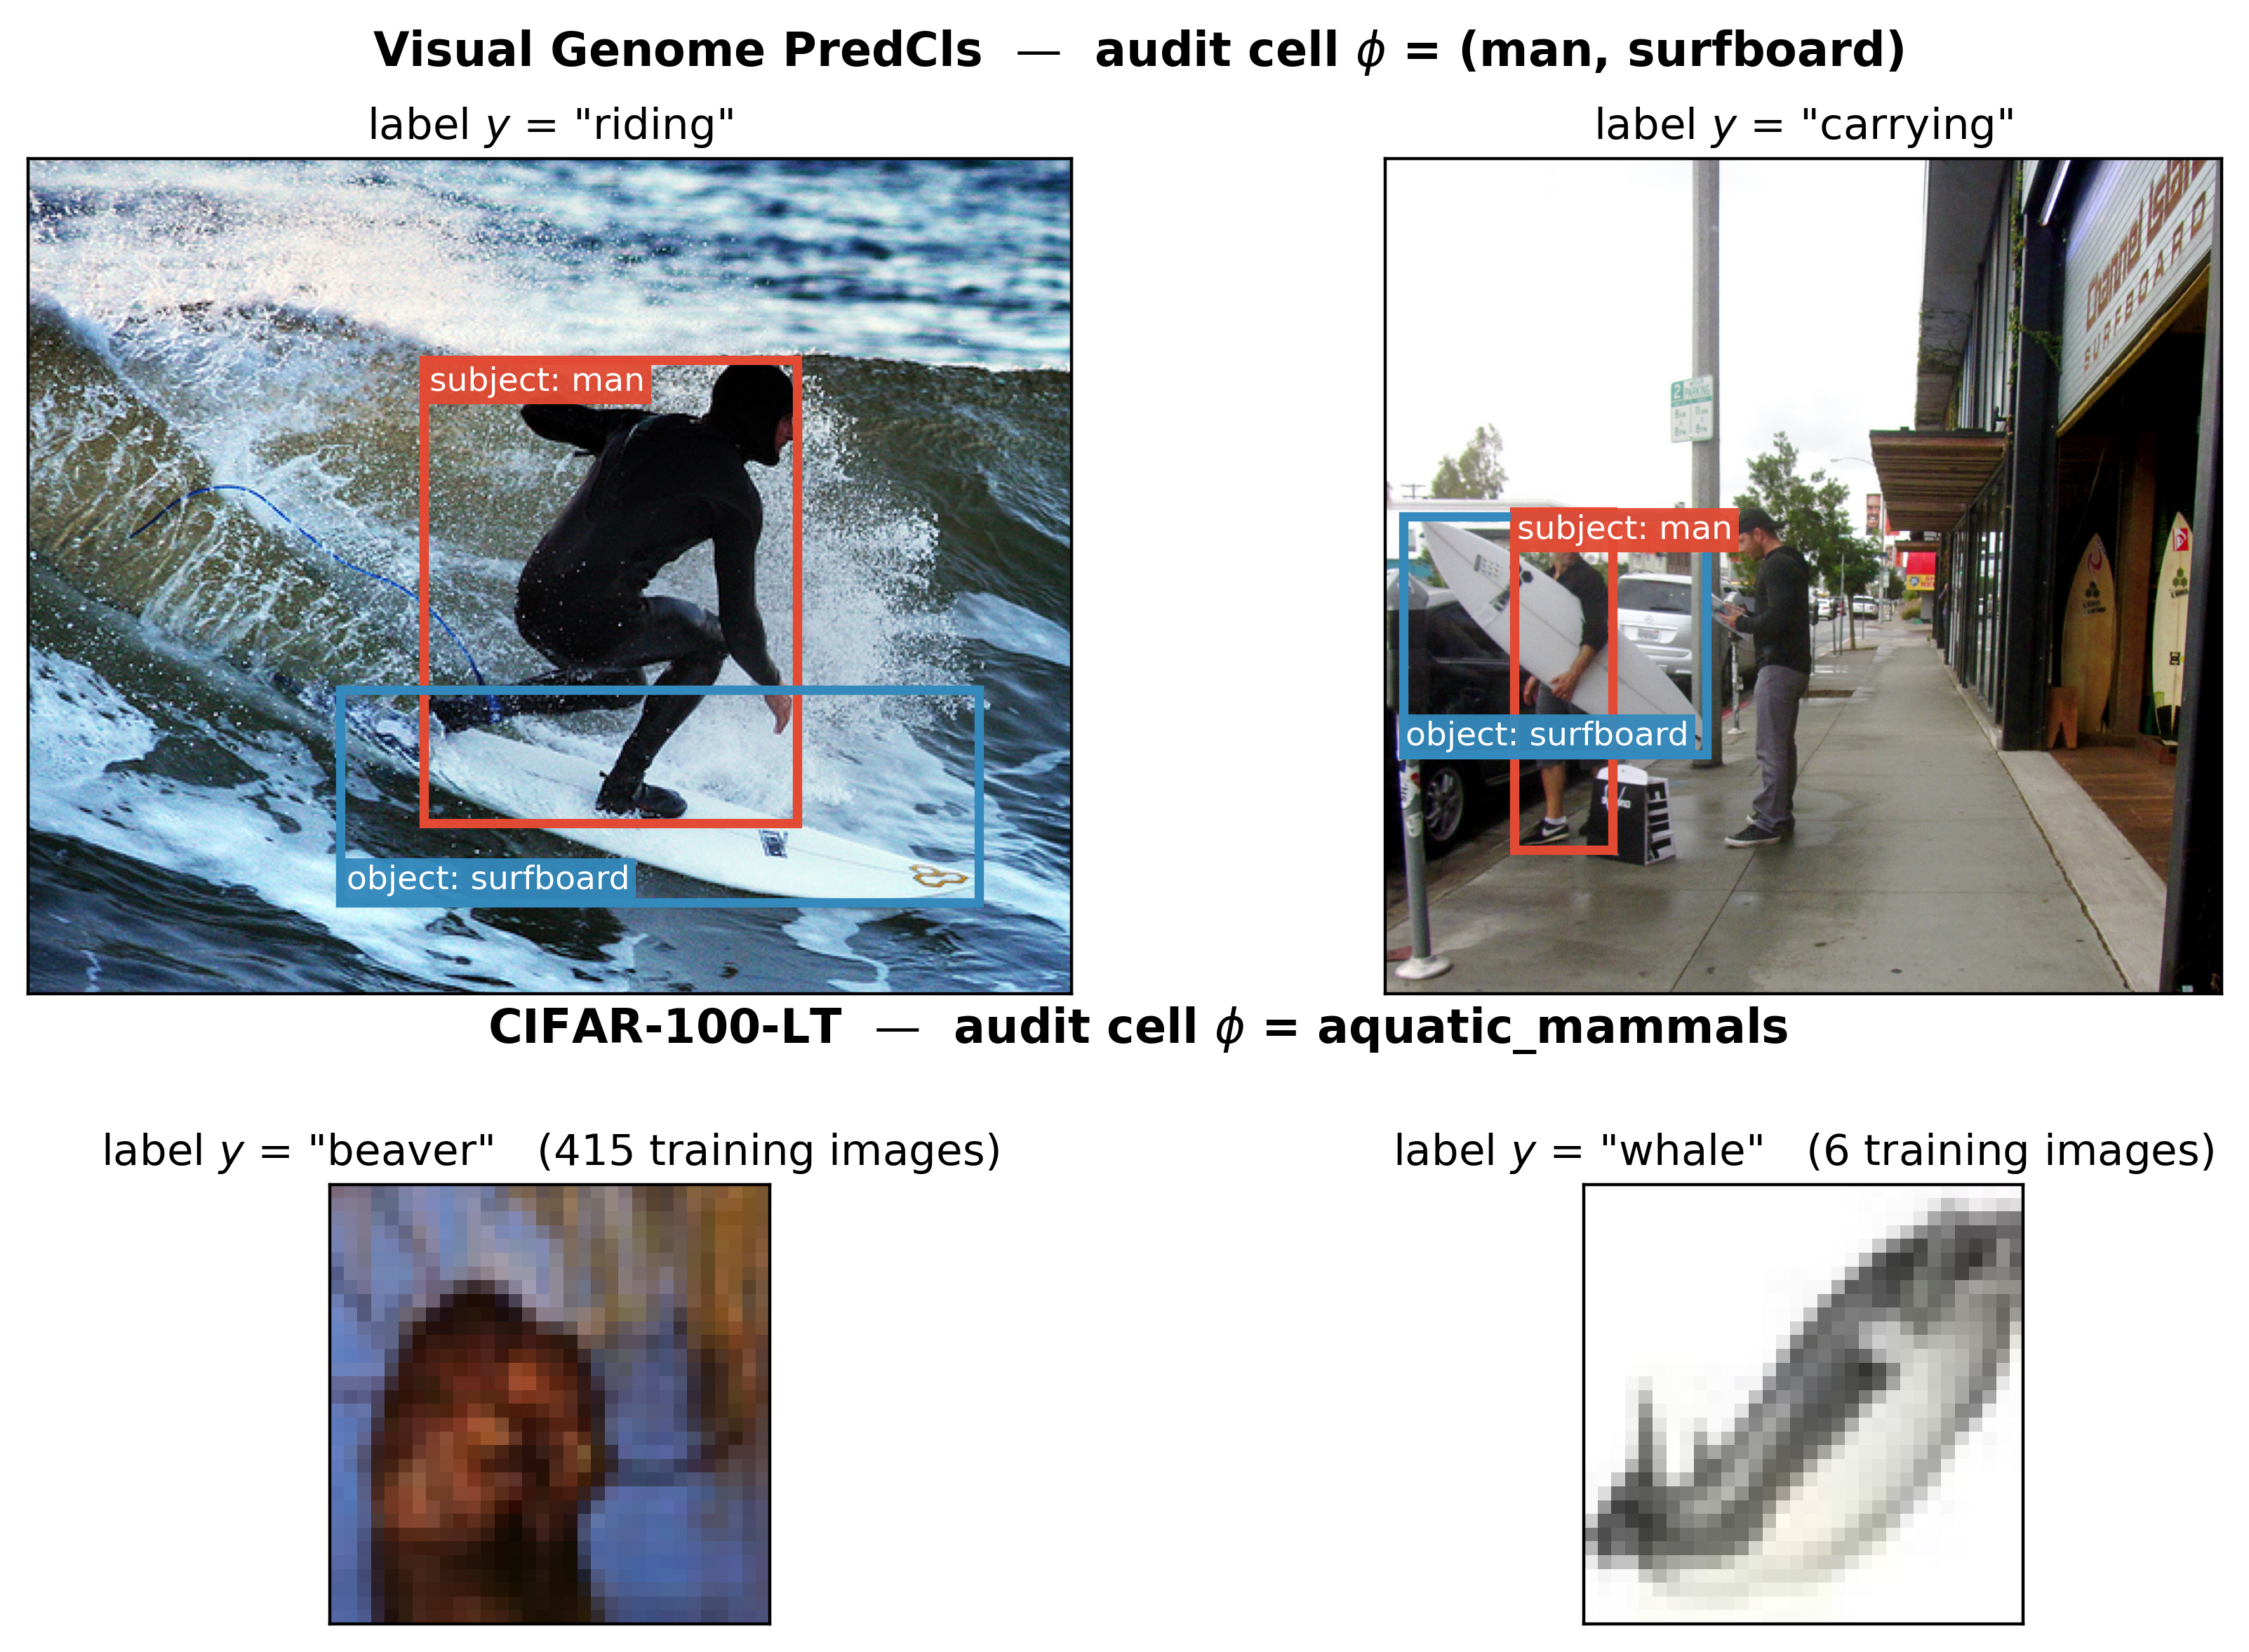
\includegraphics[width=\textwidth]{figures/fig6_dataset_samples.png}
\caption{\textbf{What a cell contains, on both benchmarks.} Each row shows two
real test examples that share the same declared grouping variable $\phi$ but carry
different labels -- precisely the configuration within-cell transport exploits.
\emph{Top:} two Visual Genome relations from the cell $\phi=(\text{man},
\text{surfboard})$. The class pair is identical and therefore cannot distinguish
``riding'' from ``carrying''; only the image content can, which is what
$\Delta R$ is designed to credit. Boxes are the annotated subject (red) and object
(blue) regions that MLP-SPATIAL turns into geometry features and MLP-VISUAL crops and
encodes with CLIP. \emph{Bottom:} two CIFAR-100 test images from the superclass
$\phi=\text{aquatic\_mammals}$, drawn from opposite ends of the long-tailed training
distribution ($415$ versus $6$ training images). Crossing the labels within a row
preserves the cell and its label histogram while destroying which prediction belongs
with which instance.}
\label{fig:samples}
\end{figure*}

\begin{table}[t]
\centering
\caption{Frozen-model top-1 accuracy on VG150 PredCls. Similar accuracies do not reveal
whether the difference is transported.}
\label{tab:accuracy}
\begin{tabular}{@{}lr@{}}
\toprule
Model & Accuracy \\
\midrule
FREQ & 0.6564 \\
FREQ+OVERLAP & 0.6545 \\
MLP-CLASS & 0.6554 \\
MLP-SPATIAL & 0.6639 \\
MLP-SPATIAL+ & 0.6674 \\
\bottomrule
\end{tabular}
\end{table}

\subsection{Gain attribution for the controlled predictors}\label{sec:results}

The central result is collected in Table~\ref{tab:wager-results} and
Figure~\ref{fig:results}. MLP-CLASS improves on FREQ by $0.03386$ of quadratic score,
yet because its gain vector is constant inside every class-pair cell, the estimator
assigns that entire improvement to prior transport and precisely nothing to instance
covariance. The zero is worth dwelling on: it follows algebraically from the construction
rather than from a learned baseline happening to pass a sanity check.

Adding box geometry changes the picture. MLP-SPATIAL gains $0.04270$ over FREQ, of which
$0.02832$ survives label transport and $0.01439$ is within-group covariance (CI
$[0.01373,0.01504]$). More revealing still is the direct comparison against MLP-CLASS,
where the total gain falls to $0.00885$ only because the transported channel deteriorates by
$0.00554$ even as the covariance gain from spatial features rises by $0.01439$. The resulting covariance share
of 1.63 records a genuinely useful instance-specific change that the aggregate score
partly conceals behind a worse prior component, and it is exactly the configuration that
a ratio confined to $[0,1]$, or thresholded at $0.5$, would misdescribe.

The remaining two comparisons bracket the interesting range. MLP-SPATIAL+ adds $0.00374$
over MLP-SPATIAL, nearly all of it covariance gain at $0.00321$ (CI $[0.00289,0.00353]$),
whereas FREQ+OVERLAP supplies the opposite caution: its overlap indicator does create a
small positive covariance gain, but the accompanying negative prior term is larger, so
the model ends up worse overall. Using image-derived information is thus never treated
as an improvement in itself; both channels are reported, signs included.

\paragraph{Reading the magnitudes.} Quadratic-score units are not ones most readers
calibrate by eye, so it is worth anchoring them in the rank-based metrics this
literature reports. Where both channels point the same way the correspondence is
straightforward: MLP-SPATIAL-S's $\widehat{\Delta R}=+0.01023$ over MLP-CLASS-S
accompanies $+0.51$ points of top-1 predicate accuracy, $+0.60$ of mean reciprocal rank
and $+0.86$ of recall@5, so in these data a hundredth of quadratic-score gain is worth
roughly half an accuracy point. The covariance channel is not, however, a re-description
of any rank metric, and the real-pixel comparison of Section~\ref{sec:vgvisual} is
where that becomes visible: there $\widehat{\Delta R}=+0.00641$ while top-1 accuracy
falls by $3.07$ points and recall@5 by $2.21$. Prior-matching both models before scoring
narrows the accuracy gap to $2.17$ points without closing it. The rank metrics aggregate
the two channels into one number; when the channels carry opposite signs, as they do
here, no single such number can represent both, which is precisely the situation the
decomposition exists to report.

\begin{table*}[t]
\centering
\caption{WAGER decomposition on 227,337 identified VG150 PredCls relations. Gains use
the quadratic score. CI is image-cluster robust; $p$ is the 499-shift relation-level
randomization diagnostic (granularity floor $.002$). ``--'' denotes an undefined share
because total gain is negative. The MLP-CLASS row's zero-width interval is exact by
construction, not a sampling statement: a gain vector constant within every cell makes
the antisymmetric kernel identically zero (Theorem~\ref{thm:population}), so no
variability exists for the interval to measure.}
\label{tab:wager-results}
\resizebox{\textwidth}{!}{%
\begin{tabular}{@{}llrrrrr@{}}
\toprule
New model & Old model & $\widehat{\Delta T}$ & $\widehat{\Delta P}$ &
$\widehat{\Delta R}$ (95\% CI) & $\widehat\rho$ & $p$ \\
\midrule
FREQ+OVERLAP & FREQ & $-0.01229$ & $-0.01430$ & $0.00202\,[0.00168,0.00235]$ & -- & .002 \\
MLP-CLASS & FREQ & $0.03386$ & $0.03386$ & $0.00000\,[0.00000,0.00000]$ & 0.00 & .724 \\
MLP-SPATIAL & FREQ & $0.04270$ & $0.02832$ & $0.01439\,[0.01373,0.01504]$ & 0.34 & .002 \\
MLP-SPATIAL+ & FREQ & $0.04644$ & $0.02885$ & $0.01760\,[0.01686,0.01834]$ & 0.38 & .002 \\
MLP-SPATIAL & MLP-CLASS & $0.00885$ & $-0.00554$ & $0.01439\,[0.01373,0.01504]$ & 1.63 & .002 \\
MLP-SPATIAL+ & MLP-SPATIAL & $0.00374$ & $0.00053$ & $0.00321\,[0.00289,0.00353]$ & 0.86 & .002 \\
\bottomrule
\end{tabular}
}
\end{table*}

\begin{figure*}[t]
\centering
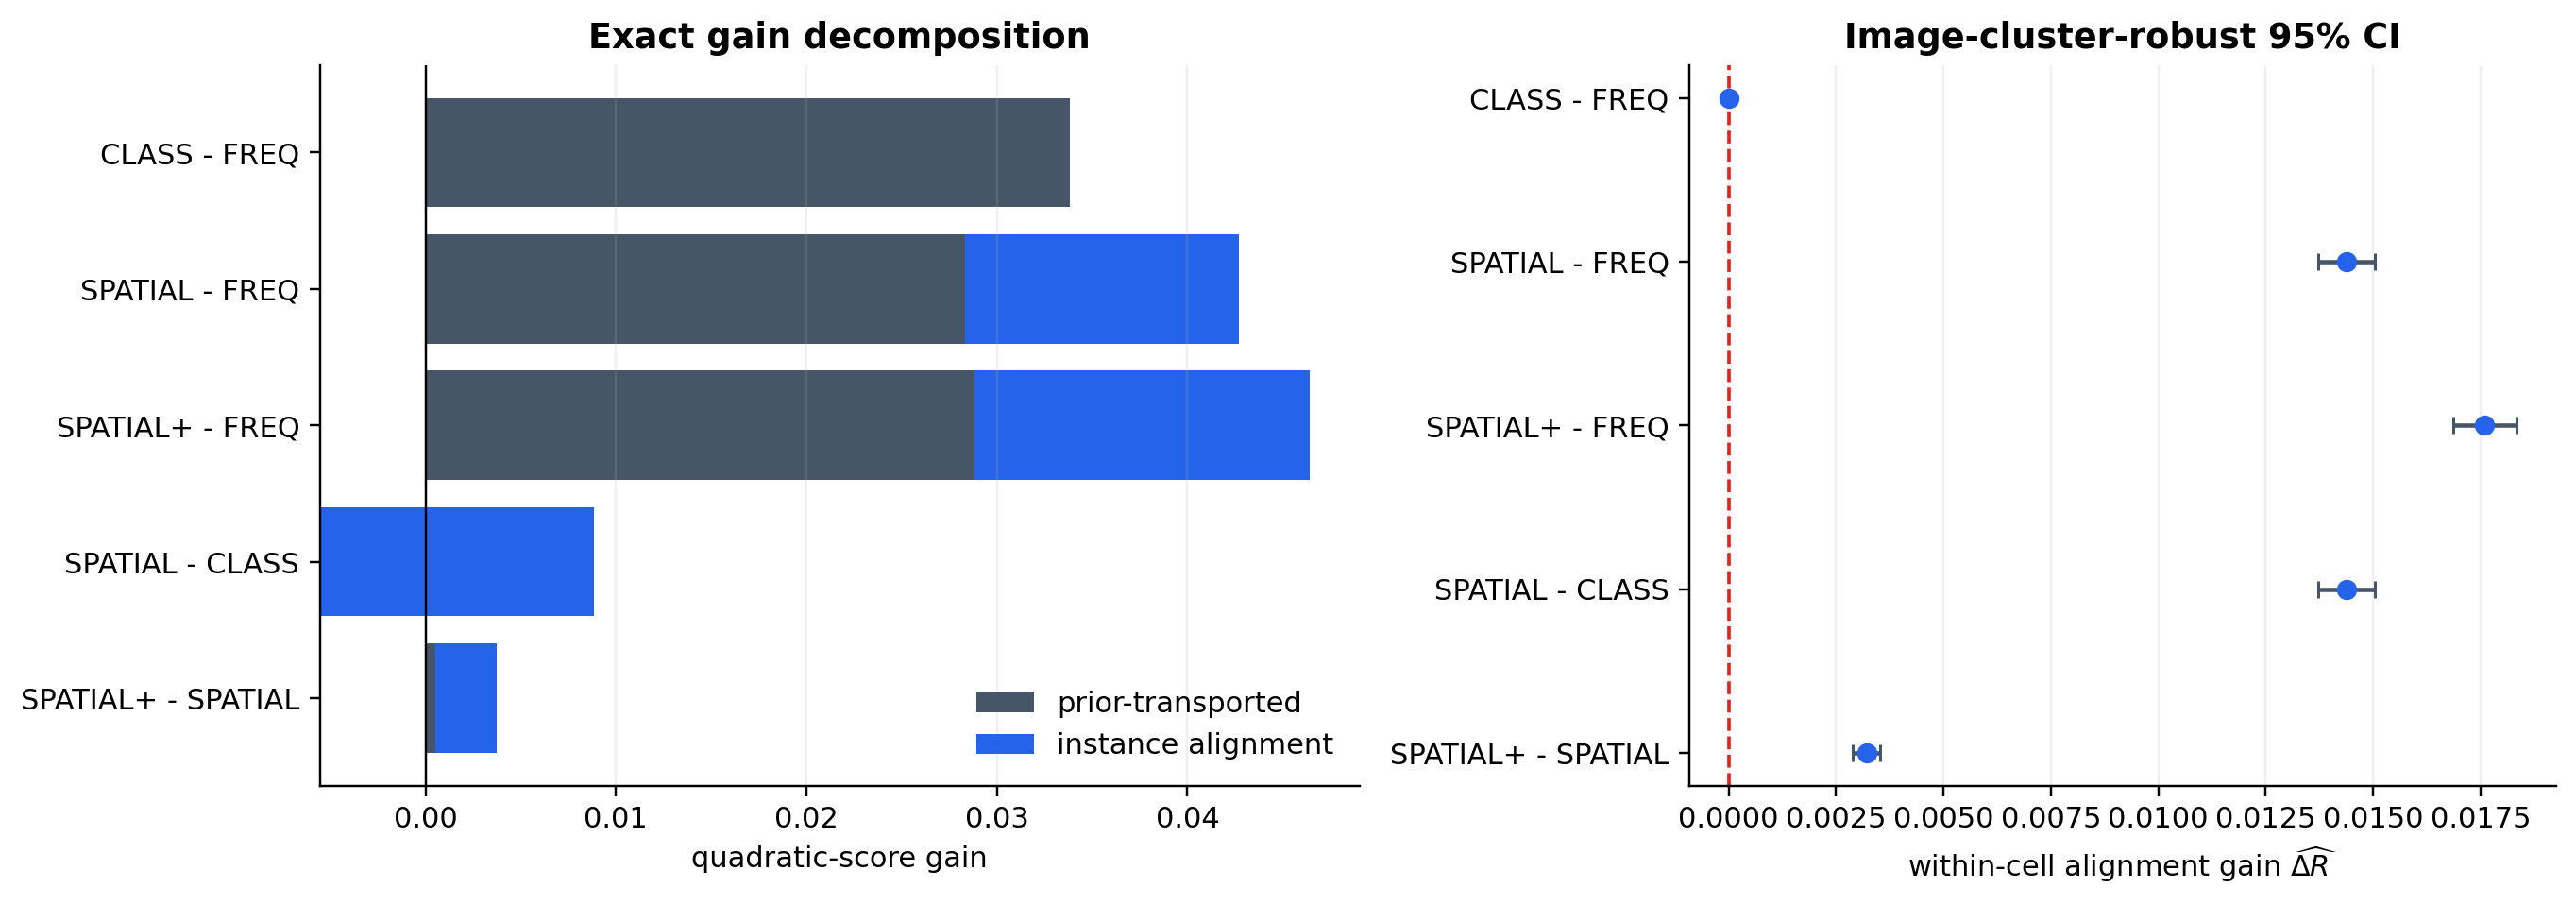
\includegraphics[width=\textwidth]{figures/fig4_new_results.png}
\caption{\textbf{Direct model-pair attribution.} Left: exact decomposition of each
positive gain into transported and within-group covariance components (the negative
prior term for SPATIAL--CLASS extends left of zero). Right: primary covariance estimates
with image-cluster-robust intervals.}
\label{fig:results}
\end{figure*}

\paragraph{Reading $\widehat{\Delta T}$ as a comparative forecast test.}
Corollary~\ref{cor:dm} identifies $\widehat{\Delta T}$ and its image-clustered interval in Table
\ref{tab:wager-results} as a grouped Diebold--Mariano statistic and interval, on the identified subsample, for
each pair's paired score differential, so every row already reports what that classical
test would report. What it does not report is the next two columns: whether MOTIFS-TDE
(Section~\ref{sec:sggaudit}) or MLP-SPATIAL beat their baseline for a reason a
frequency-only remodeling of the same benchmark could not reproduce, which is the
question $\widehat{\Delta P}$ and $\widehat{\Delta R}$ answer and DM/GW do not ask.


\subsection{Real pixels against a geometric proxy, in full}\label{app:vgvisual-full}

None of the predictors above ever sees an image: they are functions of the class pair and,
for MLP-SPATIAL(+), of box coordinates recorded in the annotation. Since box geometry is
only a proxy for image content, a sceptical reader may ask whether the covariance channel
responds to pixel evidence or merely to that proxy. Figure~\ref{fig:samples} sharpens the
question --- the cell $\phi=(\text{man},\text{surfboard})$ holds both ``riding'' and
``carrying'', and what distinguishes them is what the photograph shows.

MLP-VISUAL answers it. Subject and object regions are cropped from the original image and
each encoded by a frozen CLIP ViT-B/32 encoder \citep{radford2021learning}; the two
$512$-dimensional embeddings are concatenated with the class embeddings MLP-CLASS already
uses and passed to a small trained head. Because CLIP is never fine-tuned, whatever
covariance the model gains reflects information its pretraining already recovered from
pixels rather than representation learning on Visual Genome.

Encoding every training relation with CLIP is expensive, so MLP-VISUAL must be trained on a
subsample; setting a subsampled model against the full-data MLP-SPATIAL would confound
feature content with training-set size. All three compared predictors are therefore
retrained on one fixed, seeded subsample of $100{,}000$ of the $532{,}987$ training
relations, written MLP-CLASS-S, MLP-SPATIAL-S and MLP-VISUAL-S, so any gap between them
isolates the features. The audit still uses the full $229{,}605$-relation test split with
the same class-pair $\phi$ and image-clustered intervals.

\paragraph{Result.} By any aggregate measure the CLIP model is the worst of the three: top-1
accuracy $0.6161$ against $0.6467$ for MLP-SPATIAL-S and $0.6416$ for MLP-CLASS-S, and a
quadratic score $0.04655$ below MLP-SPATIAL-S. An evaluator reading either number would
discard it.

The decomposition contradicts that reading on the axis that matters. Against MLP-SPATIAL-S
the CLIP model loses $0.05296$ of transported gain while \emph{gaining} $0.00641$ of
covariance (95\% CI $[0.00514,0.00769]$, randomization $p=.002$): its entire deficit sits in
the transported channel and its within-cell discrimination is significantly better, not
worse. Against the class-only baseline the point is plainer still --- pixels buy $0.01665$
of covariance where box geometry buys $0.01023$, with well-separated intervals. Real image
content carries more case-specific signal than the geometric proxy standing in for it.

A plausible mechanism, stated as hypothesis rather than finding: the $1024$ CLIP dimensions
dominate the $64$ dimensions of class embedding the head also receives, so the model fits
VG150's class-pair frequency structure markedly less well than a predictor built around it. A
benchmark whose headline metric rewards transported gain will punish this model, and the
aggregate numbers duly do. What the decomposition adds is that the punishment is not for
failing to use the image. Two falsification checks, reported in
Section~\ref{app:implementation}, support that reading: correcting a model's within-cell
prior towards the training histogram registers as almost pure transported movement
($+0.02401$ against $+0.00111$ of covariance), as a correction carrying no case-level
information must, and applied to the CLIP model it halves the aggregate deficit ($-0.04655$
to $-0.02143$) while the covariance advantage persists ($+0.00752$, and $+0.00663$ when both
models are corrected) and survives confidence matching ($+0.00467$, CI
$[+0.00314,+0.00621]$).

\begin{table}[t]
\centering
\caption{Matched-subsample real-pixel study on the full VG150 test split (coverage
$99.0\%$, as in Table~\ref{tab:wager-results}). All three predictors are trained on the
same $100{,}000$ relations and differ only in features. CI is image-cluster robust on
$\widehat{\Delta R}$; $p$ is the 499-shift randomization diagnostic.}
\label{tab:vgvisual}
\resizebox{\textwidth}{!}{%
\begin{tabular}{@{}llrrrr@{}}
\toprule
New model & Old model & $\widehat{\Delta T}$ & $\widehat{\Delta P}$ &
$\widehat{\Delta R}$ (95\% CI) & $p$ \\
\midrule
MLP-SPATIAL-S & MLP-CLASS-S   & $0.00503$  & $-0.00520$ & $0.01023\,[0.00967,0.01079]$ & .002 \\
MLP-VISUAL-S  & MLP-CLASS-S   & $-0.04152$ & $-0.05816$ & $0.01665\,[0.01534,0.01796]$ & .002 \\
MLP-VISUAL-S  & MLP-SPATIAL-S & $-0.04655$ & $-0.05296$ & $0.00641\,[0.00514,0.00769]$ & .002 \\
\bottomrule
\end{tabular}
}
\end{table}

\begin{figure*}[t]
\centering
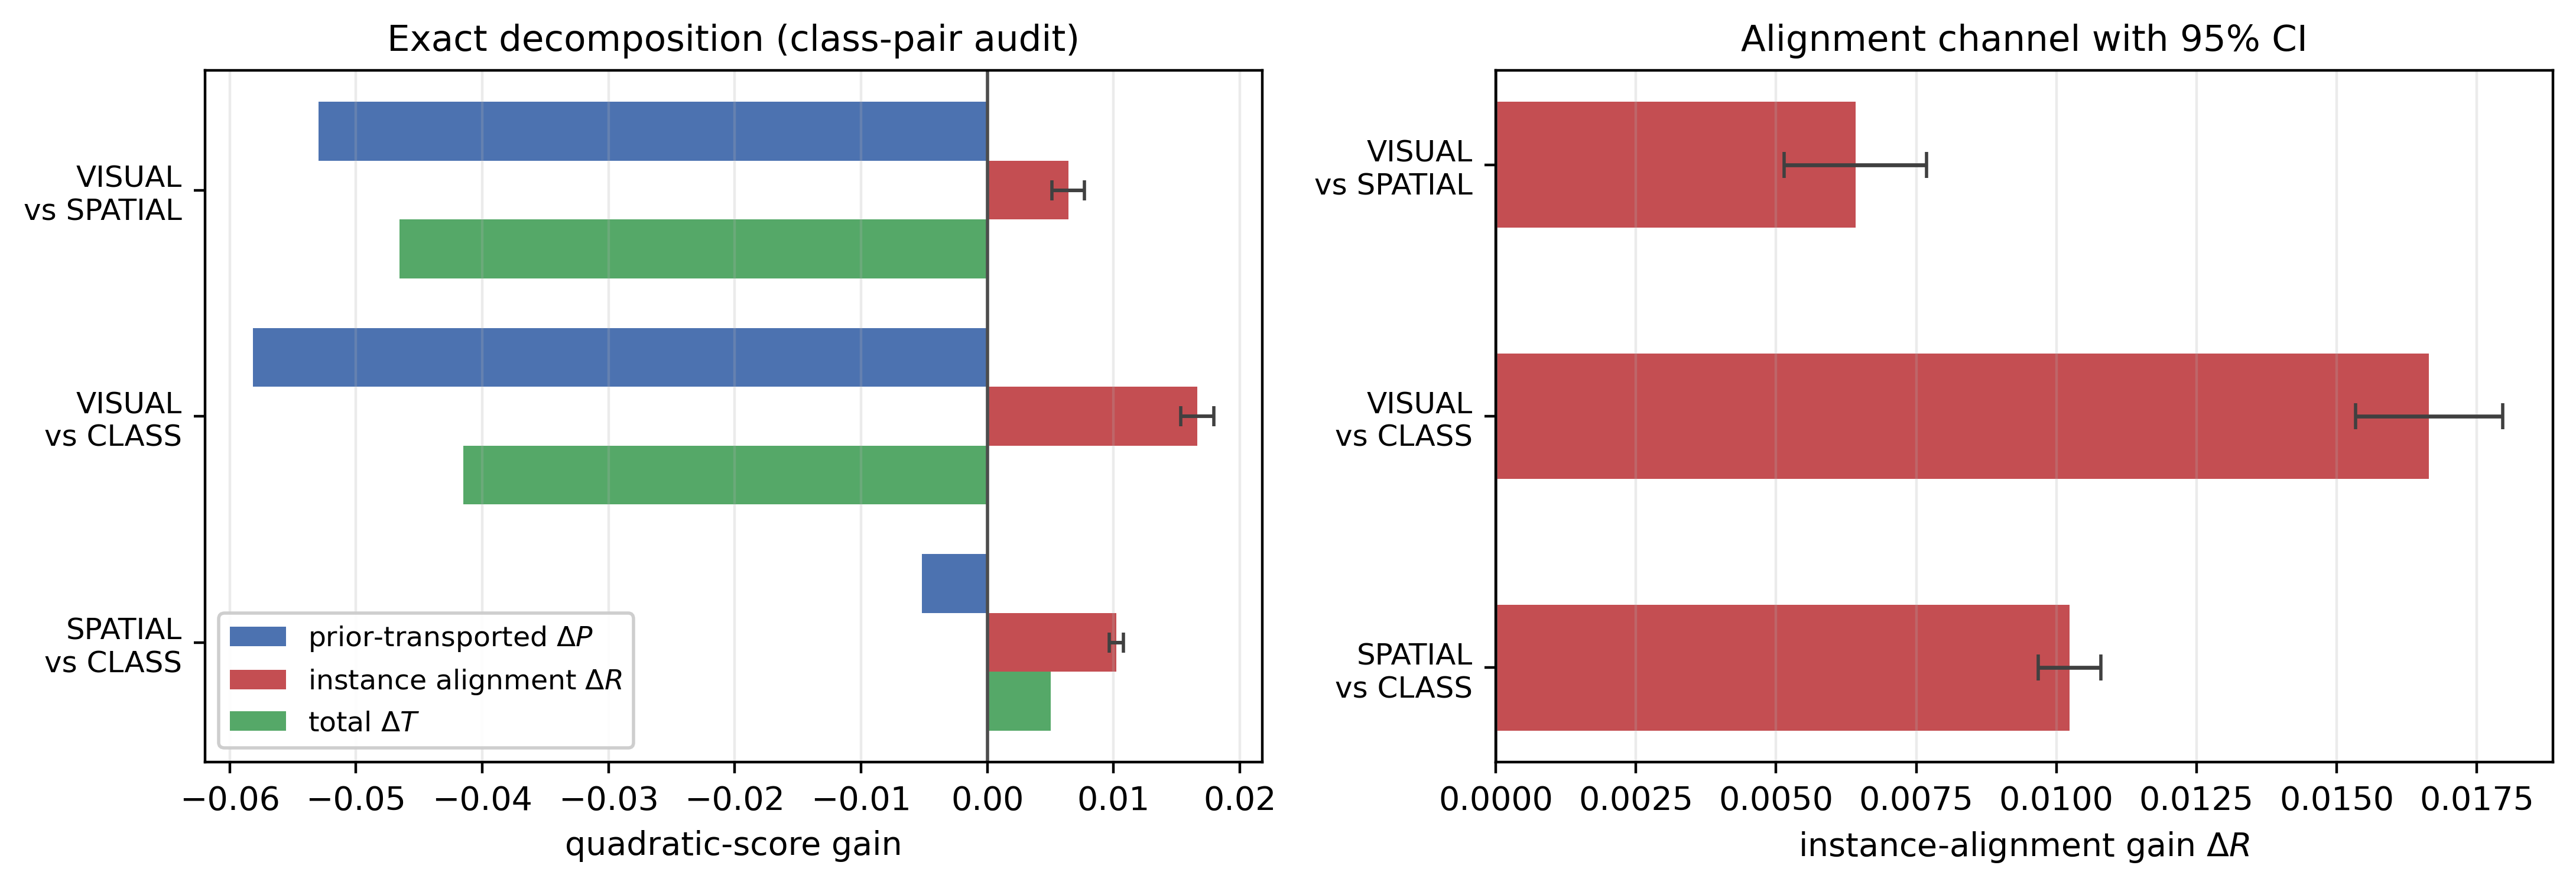
\includegraphics[width=\textwidth]{figures/fig7_vg_visual.png}
\caption{\textbf{Pixels beat geometry on covariance while losing on the aggregate.}
Left: the exact decomposition for the three matched-subsample pairs. Both comparisons
involving the CLIP model have strongly negative totals (green) driven entirely by the
transported channel (blue), while their covariance channel (red) is positive in every case.
Right: the covariance channel alone, with 95\% image-clustered intervals. Replacing box
geometry with real image content raises within-group covariance from $0.01023$ to $0.01665$
over the same class-only baseline.}
\label{fig:vgvisual}
\end{figure*}


\subsection{Sensitivity analyses}\label{sec:ablations}

For MLP-SPATIAL versus MLP-CLASS, the conclusion survives every planned sensitivity
check (Table~\ref{tab:sensitivity}). Changing from the quadratic to a probability-floored
log score changes scale ($0.01439$ to $0.06536$) but not sign or significance.
The coverage column matters for reading the rows against each other, and earlier
versions of this table omitted it. Each row targets the identified subpopulation its own
setting defines, so the minimum-cell-size rows are not four estimates of one quantity:
raising the minimum from $2$ to $20$ drops coverage from $99.0\%$ to $86.7\%$ and changes
the estimand along with the estimator. That the estimate moves so little across them
($0.01439$ to $0.01225$) is therefore mild evidence of stability rather than a
sensitivity analysis holding the target fixed.

Coarsening $\phi$ from the class pair to subject class increases the credited covariance
to $0.02181$. Proposition~\ref{prop:coarsen} identifies why: the coarser cell's estimate
equals the class-pair estimate's conditional average plus a between-class-pair covariance
term, and that term is positive here, meaning some of the credited gain reflects
class-pair-level structure that the finer audit had already correctly assigned to
$\Delta P$. This is precisely the sense in which the class-pair audit is the conservative
choice: it is not that coarsening is wrong, but that it cannot be assumed neutral, and
only the finer partition's estimate isolates covariance gain net of every prior regularity
expressible in $\phi$. The same class-pair-versus-subject-only pair also instantiates
Proposition~\ref{prop:sensitivity} directly, with the subject class playing the role of
the unrecorded confounder $Z$: Table~\ref{tab:sensitivity-numeric} in
Section~\ref{app:sensitivity} reports that the resulting bias of $0.00742$ is comfortably
inside the Cauchy--Schwarz bound, though the bound is loose enough at $K=50$ that it
would remain satisfied for a $\bar\rho$ three orders of magnitude smaller than one.
Raising the minimum cell size from 2 to 5, 10, and 20 yields
$0.01395$, $0.01330$, and $0.01225$; all cluster-robust lower limits remain positive.
The procedure itself has no smoothing strength, split fraction, or decision threshold
to tune.

\begin{table}[t]
\centering
\caption{Sensitivity of the MLP-SPATIAL vs.\ MLP-CLASS decomposition to score, audit
granularity, and minimum cell size. CI is image-cluster robust on $\widehat{\Delta R}$.}
\label{tab:sensitivity}
\small
\begin{tabular}{@{}llrr@{\,}rr@{}}
\toprule
Factor & Setting & $\widehat{\Delta T}$ & \multicolumn{1}{r}{$\widehat{\Delta R}$ (95\% CI)} & Cells &
Cov. \\
\midrule
Score & Brier (def.) & $0.00885$ & $0.01439\,[0.01373,0.01504]$ & 6346 & $99.0\%$ \\
Score & Log (floored) & $0.04297$ & $0.06536\,[0.06294,0.06779]$ & 6346 & $99.0\%$ \\
Cell $\phi$ & class pair (def.) & $0.00885$ & $0.01439\,[0.01373,0.01504]$ & 6346 & $99.0\%$ \\
Cell $\phi$ & subject only & $0.00943$ & $0.02181\,[0.02079,0.02283]$ & 150 & $100.0\%$ \\
Min.\ cell size & 2 (def.) & $0.00885$ & $0.01439\,[0.01373,0.01504]$ & 6346 & $99.0\%$ \\
Min.\ cell size & 5 & $0.00772$ & $0.01395\,[0.01329,0.01462]$ & 4060 & $96.3\%$ \\
Min.\ cell size & 10 & $0.00683$ & $0.01330\,[0.01262,0.01398]$ & 2744 & $92.6\%$ \\
Min.\ cell size & 20 & $0.00570$ & $0.01225\,[0.01155,0.01295]$ & 1757 & $86.7\%$ \\
\bottomrule
\end{tabular}
\end{table}


\subsection{Long-tailed image classification}\label{app:lt}\label{sec:cifarlt}

Sections~\ref{sec:data}--\ref{sec:vgvisual} are all instances of one task (predicate
classification on an ordered object pair). Section~\ref{sec:related-applied} argued
that long-tailed image classification poses a structurally identical question: a
class-frequency prior can be fit better without any per-instance improvement. We test
this directly on CIFAR-100-LT \citep{cui2019classbalanced}, an exponential-imbalance
(ratio $100$) subsample of CIFAR-100's training split with the original, balanced test
split retained for evaluation. We train ResNet-32 \citep{he2016deep} classifiers that
differ only in their per-class loss weighting: a vanilla cross-entropy baseline (CE);
class-balanced effective-number re-weighting applied from initialization (CB)
\citep{cui2019classbalanced}; and the same re-weighting deferred to the final twenty
epochs (DRW) \citep{cao2019learning}. Optimizer, schedule, augmentation, epoch budget,
and seed are identical across runs (Section~\ref{app:implementation}).

\paragraph{Choosing $\phi$.} A declared grouping variable has to predict the label without
determining it, and this second benchmark makes the constraint unusually easy to
violate. Were $\phi$ taken to be the fine class label itself, every cell would be
label-homogeneous, within-cell transport would have nothing to cross, and
$\widehat{\Delta R}$ would come out identically zero -- an algebraic artifact wearing the
appearance of a finding. CIFAR-100's own 20 coarse superclasses avoid this, each
gathering five fine labels into a cell of $500$ balanced test images, which is
structurally the situation of a VG class-pair cell holding several predicates
(Figure~\ref{fig:samples}). Alongside the superclass audit we report two further
declared priors: the trivial coarsening to a single global cell, which audits against
the global class marginal and so instantiates Proposition~\ref{prop:coarsen} in a second
domain, and a partition into head, medium and tail training-frequency tiers. CIFAR-100
test images are independent, unlike the several relations VG draws from one photograph,
so no cluster grouping is required and the plain H\'ajek interval of
Section~\ref{sec:inference} applies directly. One semantic point matters in this domain:
transport uses each cell's \emph{test} label histogram, which on CIFAR-100-LT is
balanced. A positive $\Delta P$ here therefore records movement \emph{toward} the
balanced test marginal -- undoing the training-frequency skew -- which is precisely the
adjustment long-tailed evaluation is designed to reward; a transported gain is a
description of where score was earned, not an accusation
(Section~\ref{sec:discussion}).

\paragraph{Result.} The three classifiers reach top-1 accuracies of $0.3662$ (CE),
$0.2627$ (CB) and $0.3874$ (DRW), so re-weighting from initialization degrades the
classifier substantially while the deferred schedule delivers the improvement it was
designed to produce. Table~\ref{tab:cifar} decomposes both gains against the superclass
audit.

Of the two, the class-balanced run is the more instructive, precisely because its
aggregate score conceals almost everything of interest. On the quadratic score it gains
$+0.00143$ over the baseline, a difference small enough that a reader working from the
headline number alone would reasonably conclude that re-weighting had changed very
little. The decomposition tells another story: within superclasses the
transported channel improves by $+0.19713$ while within-group covariance deteriorates
by $-0.19569$ (95\% CI $[-0.20728,-0.18411]$), so the near-zero total is not a small
effect but two large ones that happen to cancel.

\paragraph{A calibration-matched regime.} A channel split of that shape could, however,
be produced by confidence scaling alone. Under the quadratic score the covariance channel
is a covariance between probability movements and labels
(Eq.~\eqref{eq:cov-id}), and a monotone recalibration moves it: softening an
overconfident model transfers score mass from the covariance channel to the transported channel while
adding no information about any individual image. The baseline invites exactly this
concern, assigning a mean maximum probability of $0.764$ while being correct on only
$0.3662$ of the test set. We therefore repeat the audit in a calibration-matched regime:
each model's temperature is chosen by held-out likelihood on a calibration half of the
test split ($T^*=2.85$ for CE, $3.51$ for CB, $2.61$ for DRW), the decomposition is
computed on the disjoint audit half, and the whole procedure is repeated over twenty
random splits (Table~\ref{tab:cifar-cal}). The regime's necessity is quantified by its
control row: recalibrating the baseline alone -- a transformation carrying no instance
information -- moves the channels by $+0.380$ (prior) and $-0.175$ (covariance), so the
raw split does mix calibration with discrimination.

The calibration-matched rows then separate the two schedules cleanly, and more sharply
than the raw ones. CB's covariance deficit does not shrink but widens, to
$-0.23991\,(0.00491)$: the model re-weighted from initialization has genuinely lost
within-superclass discrimination -- a real degradation that the ten-point accuracy drop
records independently -- and its near-zero raw total reflects that loss offset by its
softer, better-calibrated confidence. DRW inverts the reading its raw split suggests.
Raw, its $+0.06712$ gain divides roughly two-thirds transported to one-third covariance gain;
calibration-matched, the improvement is $+0.02173\,(0.00275)$ of which
$+0.01957\,(0.00329)$ is within-group covariance while the transported channel is close to zero
($+0.00216\,(0.00410)$). What survives calibration matching is precisely the component
the deferred schedule was designed to buy -- per-instance discrimination, concentrated
on rare classes (Table~\ref{tab:cifar-tier}) -- while the apparently transported
share of its raw gain was largely the calibration difference between the two runs.
Neither an accuracy difference nor an aggregate score exposes either composition, which
is the practical argument for reporting the two channels, in both regimes, instead of
their sum.

\begin{table}[t]
\centering
\caption{Raw and calibration-matched decompositions on CIFAR-100-LT at the superclass
audit. Temperatures are fitted by likelihood on a held-out calibration half of the test
split; every decomposition uses the disjoint audit half; entries are means (sd) over
twenty random splits. The final row is the control: recalibrating the baseline alone
carries no instance information yet moves both channels substantially.}
\label{tab:cifar-cal}
\resizebox{\textwidth}{!}{%
\begin{tabular}{@{}llrrr@{}}
\toprule
Comparison & Regime & $\widehat{\Delta T}$ & $\widehat{\Delta P}$ &
$\widehat{\Delta R}$ \\
\midrule
CB vs CE  & raw                 & $+0.00208\,(0.00642)$ & $+0.19635\,(0.00369)$ & $-0.19427\,(0.00632)$ \\
CB vs CE  & calibration-matched & $-0.12912\,(0.00373)$ & $+0.11079\,(0.00372)$ & $-0.23991\,(0.00491)$ \\
DRW vs CE & raw                 & $+0.06712\,(0.00865)$ & $+0.04258\,(0.00463)$ & $+0.02454\,(0.00685)$ \\
DRW vs CE & calibration-matched & $+0.02173\,(0.00275)$ & $+0.00216\,(0.00410)$ & $+0.01957\,(0.00329)$ \\
\midrule
CE recalibrated vs CE & control & $+0.20495\,(0.00420)$ & $+0.37960\,(0.00268)$ & $-0.17464\,(0.00455)$ \\
\bottomrule
\end{tabular}
}
\end{table}

\paragraph{Seeds, imbalance ratios, and a post-hoc arm.} A decomposition computed from
one trained pair carries only test-set sampling uncertainty, which is not the uncertainty
relevant to a claim about a training \emph{method}. We therefore retrained the triple at
two further seeds at the primary ratio and at imbalance ratios $10$ and $50$, and added a
fourth arm: post-hoc logit adjustment (LA), which divides the baseline's predictions by
the training class prior without retraining \citep{menon2021long}. Every configuration is
audited in both regimes; Table~\ref{tab:cifar-robust} reports the calibration-matched
covariance channel, which is the one the preceding paragraphs interpret.

Three things follow. First, the class-balanced run's covariance loss is not a
misconfiguration but a systematic function of imbalance severity: $-0.069$ at ratio $10$,
$-0.244$ at $50$, and $-0.251\,(0.011)$ across three seeds at $100$, tracking an accuracy
penalty that grows from $2.3$ to $10.4$ points over the same range. Second, the deferred
schedule's covariance gain is positive at every ratio and in every seed, but its magnitude
varies roughly fourfold across seeds at ratio $100$ ($+0.007$ to $+0.031$). We therefore
report the spread rather than a seed-level interval: the direction replicates, the
magnitude is seed-sensitive, and the gap between the tight within-run intervals of
Table~\ref{tab:cifar} and this across-seed spread is exactly why a method-level claim
needs replication rather than a single audit.

Third, LA is an instructive falsification of a natural expectation. A purely post-hoc
prior correction might be expected to register as almost pure transported channel, as the
within-cell prior matching of Section~\ref{sec:vgvisual} does. It does not:
calibration-matched, LA reads as almost entirely covariance gain ($+0.022$ to $+0.038$) with a
transported channel near zero, while achieving the best balanced accuracy of any arm at every
ratio. The reason is visible in the construction. Dividing by the \emph{global} class
prior is not a within-superclass histogram move, because fine classes inside a superclass
differ in training frequency, and the correction it applies is multiplicative in each
example's own predicted probabilities --- it changes rankings where the model already
carried latent evidence. The two post-hoc corrections in this paper therefore land in
opposite channels, and correctly so: transport separates adjustments that act on the
cell's label histogram from adjustments that act on individual predictions.

\begin{table}[t]
\centering
\caption{Calibration-matched covariance gain across seeds and imbalance ratios, with
balanced test accuracy for each arm. LA is post-hoc logit adjustment applied to the
baseline. The class-balanced deficit scales with imbalance severity; the deferred
schedule's gain is positive throughout but seed-sensitive in magnitude; the post-hoc
correction lands in the covariance channel rather than the transported channel.}
\label{tab:cifar-robust}
\resizebox{\textwidth}{!}{%
\begin{tabular}{@{}llrrrrrrr@{}}
\toprule
& & \multicolumn{4}{c}{Top-1 accuracy} & \multicolumn{3}{c}{$\widehat{\Delta R}$ vs.\ CE (calibration-matched)} \\
\cmidrule(lr){3-6}\cmidrule(l){7-9}
Ratio & Seed & CE & CB & DRW & LA & CB & DRW & LA \\
\midrule
$10$  & 0 & $0.5388$ & $0.5154$ & $0.5447$ & $0.5497$ & $-0.06903$ & $+0.00617$ & $+0.02222$ \\
$50$  & 0 & $0.4256$ & $0.3242$ & $0.4399$ & $0.4550$ & $-0.24409$ & $+0.01903$ & $+0.03768$ \\
$100$ & 0 & $0.3662$ & $0.2627$ & $0.3874$ & $0.3959$ & $-0.23936$ & $+0.01987$ & $+0.03449$ \\
$100$ & 1 & $0.3614$ & $0.2287$ & $0.3762$ & $0.3877$ & $-0.26176$ & $+0.00748$ & $+0.02672$ \\
$100$ & 2 & $0.3687$ & $0.2481$ & $0.3968$ & $0.4024$ & $-0.25213$ & $+0.03124$ & $+0.03601$ \\
\midrule
\multicolumn{2}{@{}l}{$100$, mean (sd)} & & & & &
$-0.25108\,(0.01124)$ & $+0.01953\,(0.01188)$ & $+0.03241\,(0.00498)$ \\
\bottomrule
\end{tabular}
}
\end{table}

Where the covariance gain sits is visible in Table~\ref{tab:cifar-tier} and
Figure~\ref{fig:cifar} (raw regime, primary seed). For DRW it falls where the long-tail literature intends it to,
reaching $+0.09009$ on few-shot classes and $+0.06760$ on medium-shot ones, while
many-shot classes lose $-0.07624$ as the schedule shifts capacity away from the head.
The class-balanced run reproduces that same ordering with every level displaced
downward, its many-shot covariance collapsing to $-0.41977$. What the decomposition
supplies, then, is not only how much of a long-tail gain is real but where in the
frequency spectrum it was earned.

These numbers also provide an implementation check on real inputs. Computing the
within-group covariance gain directly from the identity of Eq.~\eqref{eq:cov-id}, through a
code path that shares nothing with the transport estimator, gives $-0.19530$; multiplying
by the factor $n_c/(n_c-1)$ that Proposition~\ref{prop:attenuate} predicts, at the
$n_c=500$ of a balanced superclass cell, returns $-0.195693$ against the estimator's
$-0.19569$. The identities of Theorem~\ref{thm:population} and
Proposition~\ref{prop:attenuate} are algebraic, so this verifies the implementation
rather than the theory; the point of the check is that two independent code paths agree
to the fifth decimal on real trained models, not only on the synthetic populations used
in the unit tests.

\begin{table}[t]
\centering
\caption{WAGER decomposition on the 10,000-image balanced CIFAR-100-LT test split.
Gains use the quadratic score; CI is the H\'ajek interval on $\widehat{\Delta R}$;
$p$ is the 499-shift randomization diagnostic, one-sided for a positive covariance gain, so the
value of $1.000$ on the CB rows records a covariance gain at the extreme negative end of
its randomization distribution.}
\label{tab:cifar}
\resizebox{\textwidth}{!}{%
\begin{tabular}{@{}llrrrr@{}}
\toprule
Comparison & Audit cell $\phi$ & $\widehat{\Delta T}$ & $\widehat{\Delta P}$ &
$\widehat{\Delta R}$ (95\% CI) & $p$ \\
\midrule
CB vs CE  & superclass (20) & $0.00143$ & $0.19713$ & $-0.19569\,[-0.20728,-0.18411]$ & $1.000$ \\
CB vs CE  & global (1)      & $0.00143$ & $0.25573$ & $-0.25430\,[-0.26801,-0.24058]$ & $1.000$ \\
CB vs CE  & tier (3)        & $0.00143$ & $0.25247$ & $-0.25103\,[-0.26453,-0.23754]$ & $1.000$ \\
\midrule
DRW vs CE & superclass (20) & $0.06606$ & $0.04206$ & $0.02400\,[0.01340,0.03460]$ & $.002$ \\
DRW vs CE & global (1)      & $0.06606$ & $0.03522$ & $0.03085\,[0.01860,0.04309]$ & $.002$ \\
DRW vs CE & tier (3)        & $0.06606$ & $0.03702$ & $0.02904\,[0.01702,0.04107]$ & $.002$ \\
\bottomrule
\end{tabular}
}
\end{table}

\begin{table}[t]
\centering
\caption{Covariance gain by training-frequency tier at the primary superclass audit.
The deferred schedule concentrates its genuine per-instance improvement on rare
classes; both methods lose covariance on the head.}
\label{tab:cifar-tier}
\begin{tabular}{@{}lrrrr@{}}
\toprule
& & \multicolumn{1}{c}{CB vs CE} & \multicolumn{2}{c}{DRW vs CE} \\
\cmidrule(l){3-3}\cmidrule(l){4-5}
Tier & $n$ & $\widehat{\Delta R}$ & $\widehat{\Delta T}$ & $\widehat{\Delta R}$ \\
\midrule
Few-shot ($<20$)        & 3000 & $-0.03337$ & $0.13785$ & $0.09009$ \\
Medium-shot ($20$--$100$) & 3500 & $-0.11075$ & $0.10799$ & $0.06760$ \\
Many-shot ($>100$)      & 3500 & $-0.41977$ & $-0.03740$ & $-0.07624$ \\
\bottomrule
\end{tabular}
\end{table}

\begin{figure*}[t]
\centering
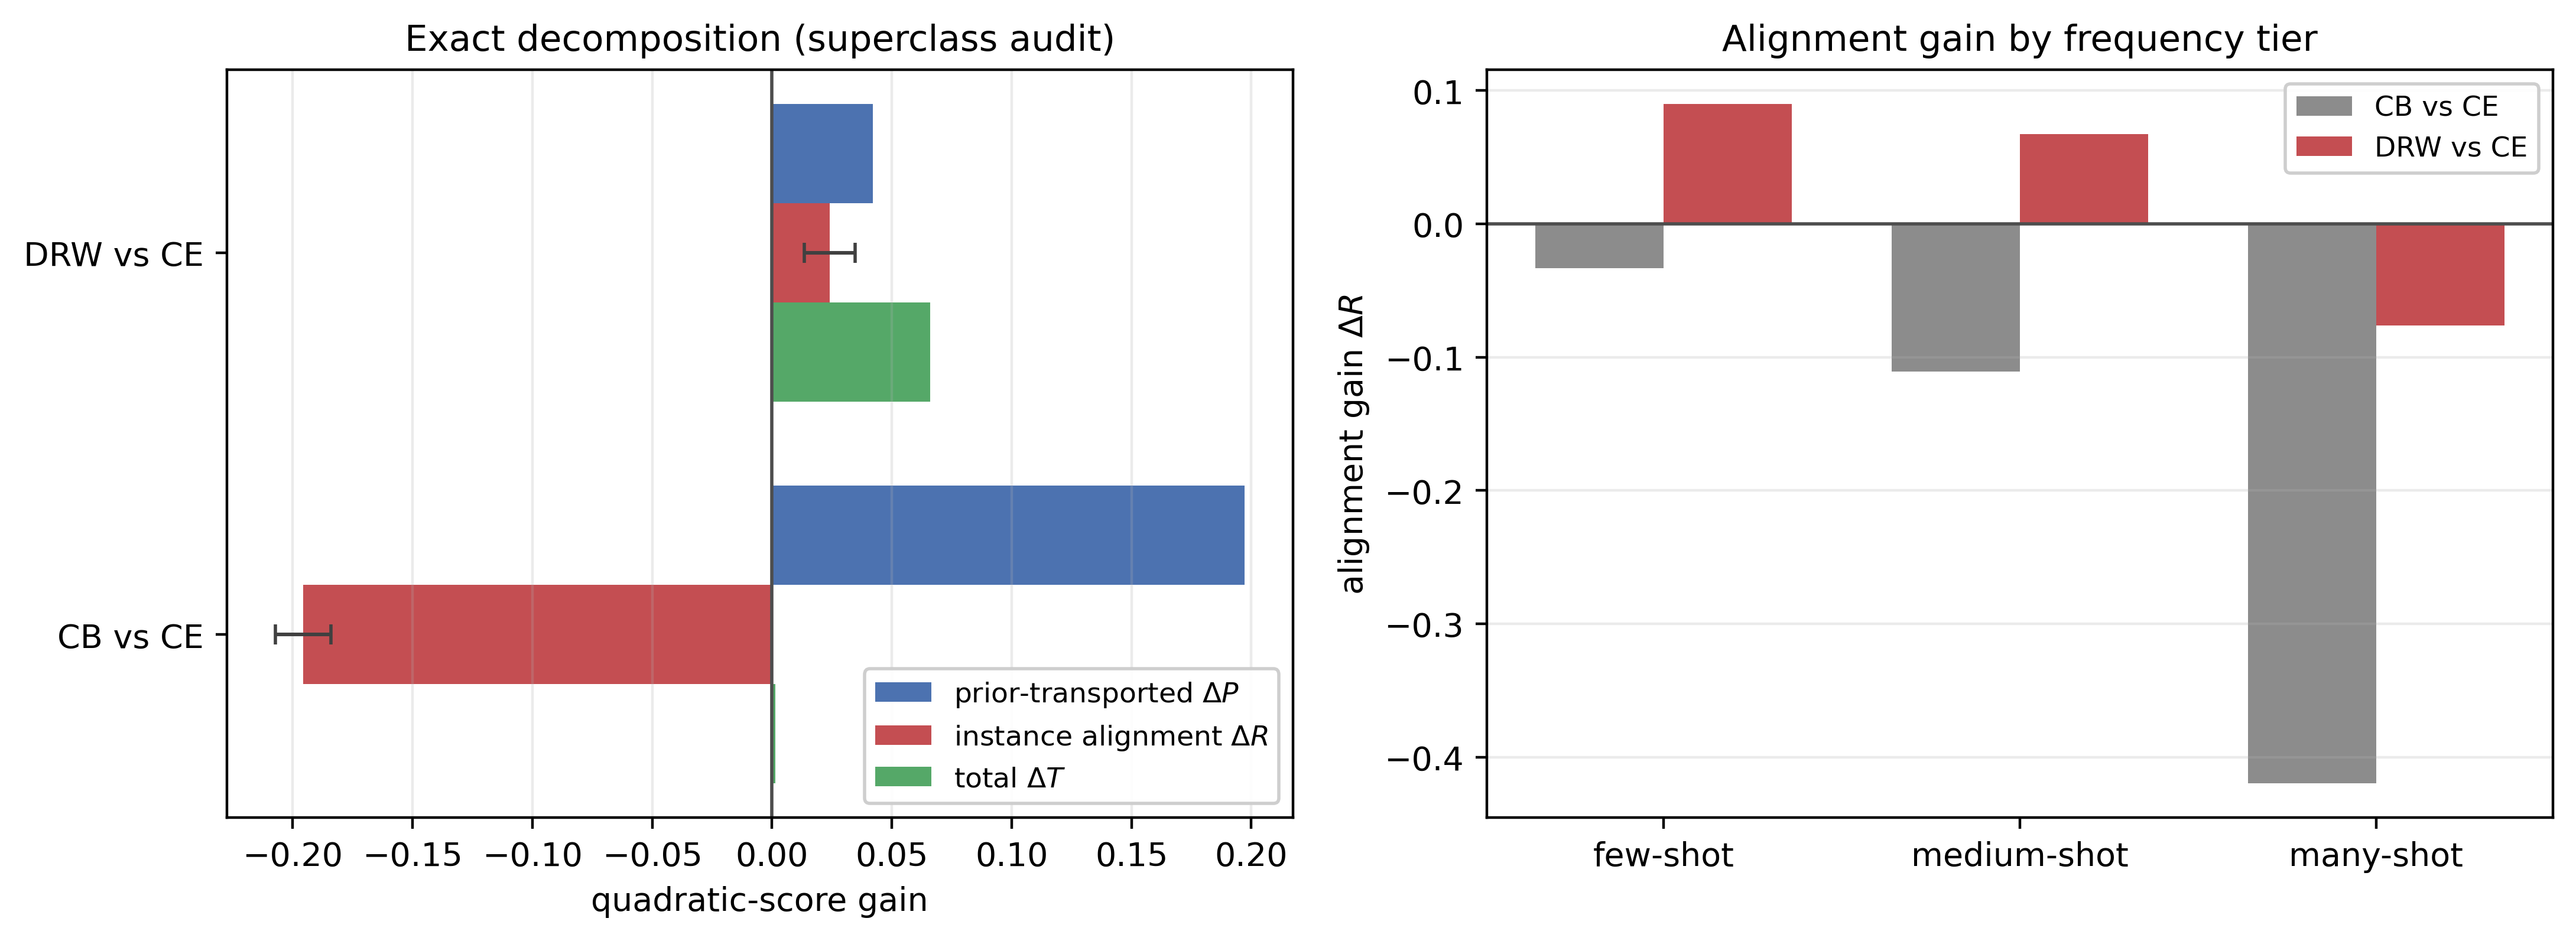
\includegraphics[width=\textwidth]{figures/fig5_cifar_lt.png}
\caption{\textbf{The same attribution transfers to a second task.} Left: exact
decomposition at the superclass audit. The CB total gain (green) is visually almost
absent at $+0.00143$ while its two channels reach $\pm0.2$ -- a near-zero aggregate
score concealing two large opposing effects. DRW's smaller total is genuinely split
between both channels. Error bars are 95\% H\'ajek intervals on $\widehat{\Delta R}$.
Right: the covariance channel by training-frequency tier, showing that DRW's genuine
per-instance gain is concentrated on rare classes and negative on the head.}
\label{fig:cifar}
\end{figure*}

Coarsening behaves as Proposition~\ref{prop:coarsen} predicts. Moving from the 20
superclass cells to a single global cell changes the credited covariance from $-0.19569$
to $-0.25430$; the difference is the between-cell covariance term, which is negative
here, so the coarse audit overstates the covariance loss by attributing to it structure
that the superclass partition correctly assigns to $\Delta P$. The finer partition is
again the conservative reading, for the same reason as in Section~\ref{sec:ablations}
and now in a second domain.

\subsection{Long-tailed text classification}\label{sec:textlt}

Sections~\ref{sec:results}--\ref{app:lt} test two vision tasks that share cached
probability vectors and grouping variables grounded in class frequency or object geometry.
To test the breadth Section~\ref{sec:discussion} claims -- any benchmark supplying two
models' full probability vectors, labels, and a declared discrete grouping variable -- we
apply the identical estimator, unmodified, to document category prediction on 20
Newsgroups \citep{lang1995newsweeder}. Neither the predictors nor the grouping variable are
visual here: documents replace images, and the declared $\phi$ is a topical grouping
rather than a spatial or class-frequency one, so a favorable result cannot be attributed
to anything specific to vision data.

We build a long-tailed training subset with the same exponential profile as
CIFAR-100-LT (imbalance ratio $100$, Section~\ref{app:lt}), applied to 20
Newsgroups' 20 fine categories, keeping the standard balanced test split ($7{,}532$
documents) untouched (Section~\ref{app:implementation}). The 20 categories fall into
six conventional coarse topics -- computing, recreation, science, politics, religion,
and classifieds -- which we use as the primary declared $\phi$, the direct analogue of
CIFAR's coarse superclasses; a global (trivial) and a training-frequency-tier partition
are reported alongside, as in Section~\ref{app:lt}. Documents are represented by a
TF-IDF vector reduced to $300$ dimensions by truncated SVD, and the three compared
classifiers -- CE, CB, and DRW -- follow the same three-arm protocol as
Section~\ref{app:lt}: an identical small MLP architecture and optimizer across runs,
differing only in per-example loss weight (Section~\ref{app:implementation}). Test
documents are independent units, so the plain H\'ajek interval of Section~\ref{sec:inference}
applies directly, as for CIFAR.

\paragraph{Result.} Table~\ref{tab:textlt} decomposes both re-weighting schedules' gain
over the cross-entropy baseline (top-1 accuracies $0.3532$ CE, $0.3960$ CB, $0.3776$
DRW). The two schedules land in opposite channels here, which is itself the finding
worth reporting: on this task it is class-balanced re-weighting from initialization, not
the deferred schedule, that buys genuine within-topic covariance gain ($+0.04317$, CI
$[0.03664,0.04970]$, $37.9\%$ of its total gain), while DRW's comparably sized total gain
($0.11490$ vs.\ CB's $0.11388$) is $98.6\%$ transported, its residual covariance
statistically indistinguishable from zero at the superclass audit ($+0.00155$, CI
$[-0.00296,0.00605]$, $p=.236$) and significantly negative once the coarser tier
partition is used instead ($-0.00901$, CI $[-0.01428,-0.00374]$). This is the reverse of
Section~\ref{app:lt}'s image-classification finding, where CB's near-zero total
masked a large covariance-gain \emph{loss} and DRW's gain was genuinely covariance-driven.
Nothing about the estimator or the construction of $\phi$ changed between the two
applications; what changed is which training recipe, on which data, buys real
per-instance discrimination -- exactly the composition question an aggregate score or an
accuracy difference alone cannot answer, now demonstrated on a domain with neither a
class-frequency table nor a spatial prior.

Coarsening moves both comparisons in the direction Proposition~\ref{prop:coarsen} allows
without requiring: CB's credited covariance falls from $0.04317$ at the superclass
partition to $0.04185$ at the global cell and $0.03578$ at the tier partition, while
DRW's changes sign twice, from a small positive residual (superclass) to a small
negative one (global) to a significant negative one (tier). None of these differences
overturns CB's conclusion, but DRW's illustrates exactly why the finest defensible
partition is the conservative default (Section~\ref{sec:coarsening}): a reader stopping
at the coarser tier partition would report a significant covariance \emph{loss} for a
method whose finer-grained residual is not distinguishable from zero.

\begin{table}[t]
\centering
\caption{WAGER decomposition on the 7,532-document balanced 20-Newsgroups-LT test
split. Gains use the quadratic score; CI is the (unclustered) H\'ajek interval on
$\widehat{\Delta R}$, documents being independent units; $p$ is the 499-shift
randomization diagnostic, one-sided for a positive covariance gain.}
\label{tab:textlt}
\resizebox{\textwidth}{!}{%
\begin{tabular}{@{}llrrrr@{}}
\toprule
Comparison & Audit cell $\phi$ & $\widehat{\Delta T}$ & $\widehat{\Delta P}$ &
$\widehat{\Delta R}$ (95\% CI) & $p$ \\
\midrule
CB vs CE  & superclass (6) & $0.11388$ & $0.07071$ & $0.04317\,[0.03664,0.04970]$ & $.002$ \\
CB vs CE  & global (1)     & $0.11388$ & $0.07203$ & $0.04185\,[0.03381,0.04990]$ & $.002$ \\
CB vs CE  & tier (3)       & $0.11388$ & $0.07810$ & $0.03578\,[0.02825,0.04331]$ & $.002$ \\
\midrule
DRW vs CE & superclass (6) & $0.11490$ & $0.11335$ & $0.00155\,[-0.00296,0.00605]$ & $.236$ \\
DRW vs CE & global (1)     & $0.11490$ & $0.11809$ & $-0.00319\,[-0.00884,0.00245]$ & $.980$ \\
DRW vs CE & tier (3)       & $0.11490$ & $0.12391$ & $-0.00901\,[-0.01428,-0.00374]$ & $1.000$ \\
\bottomrule
\end{tabular}
}
\end{table}

\begin{figure*}[t]
\centering
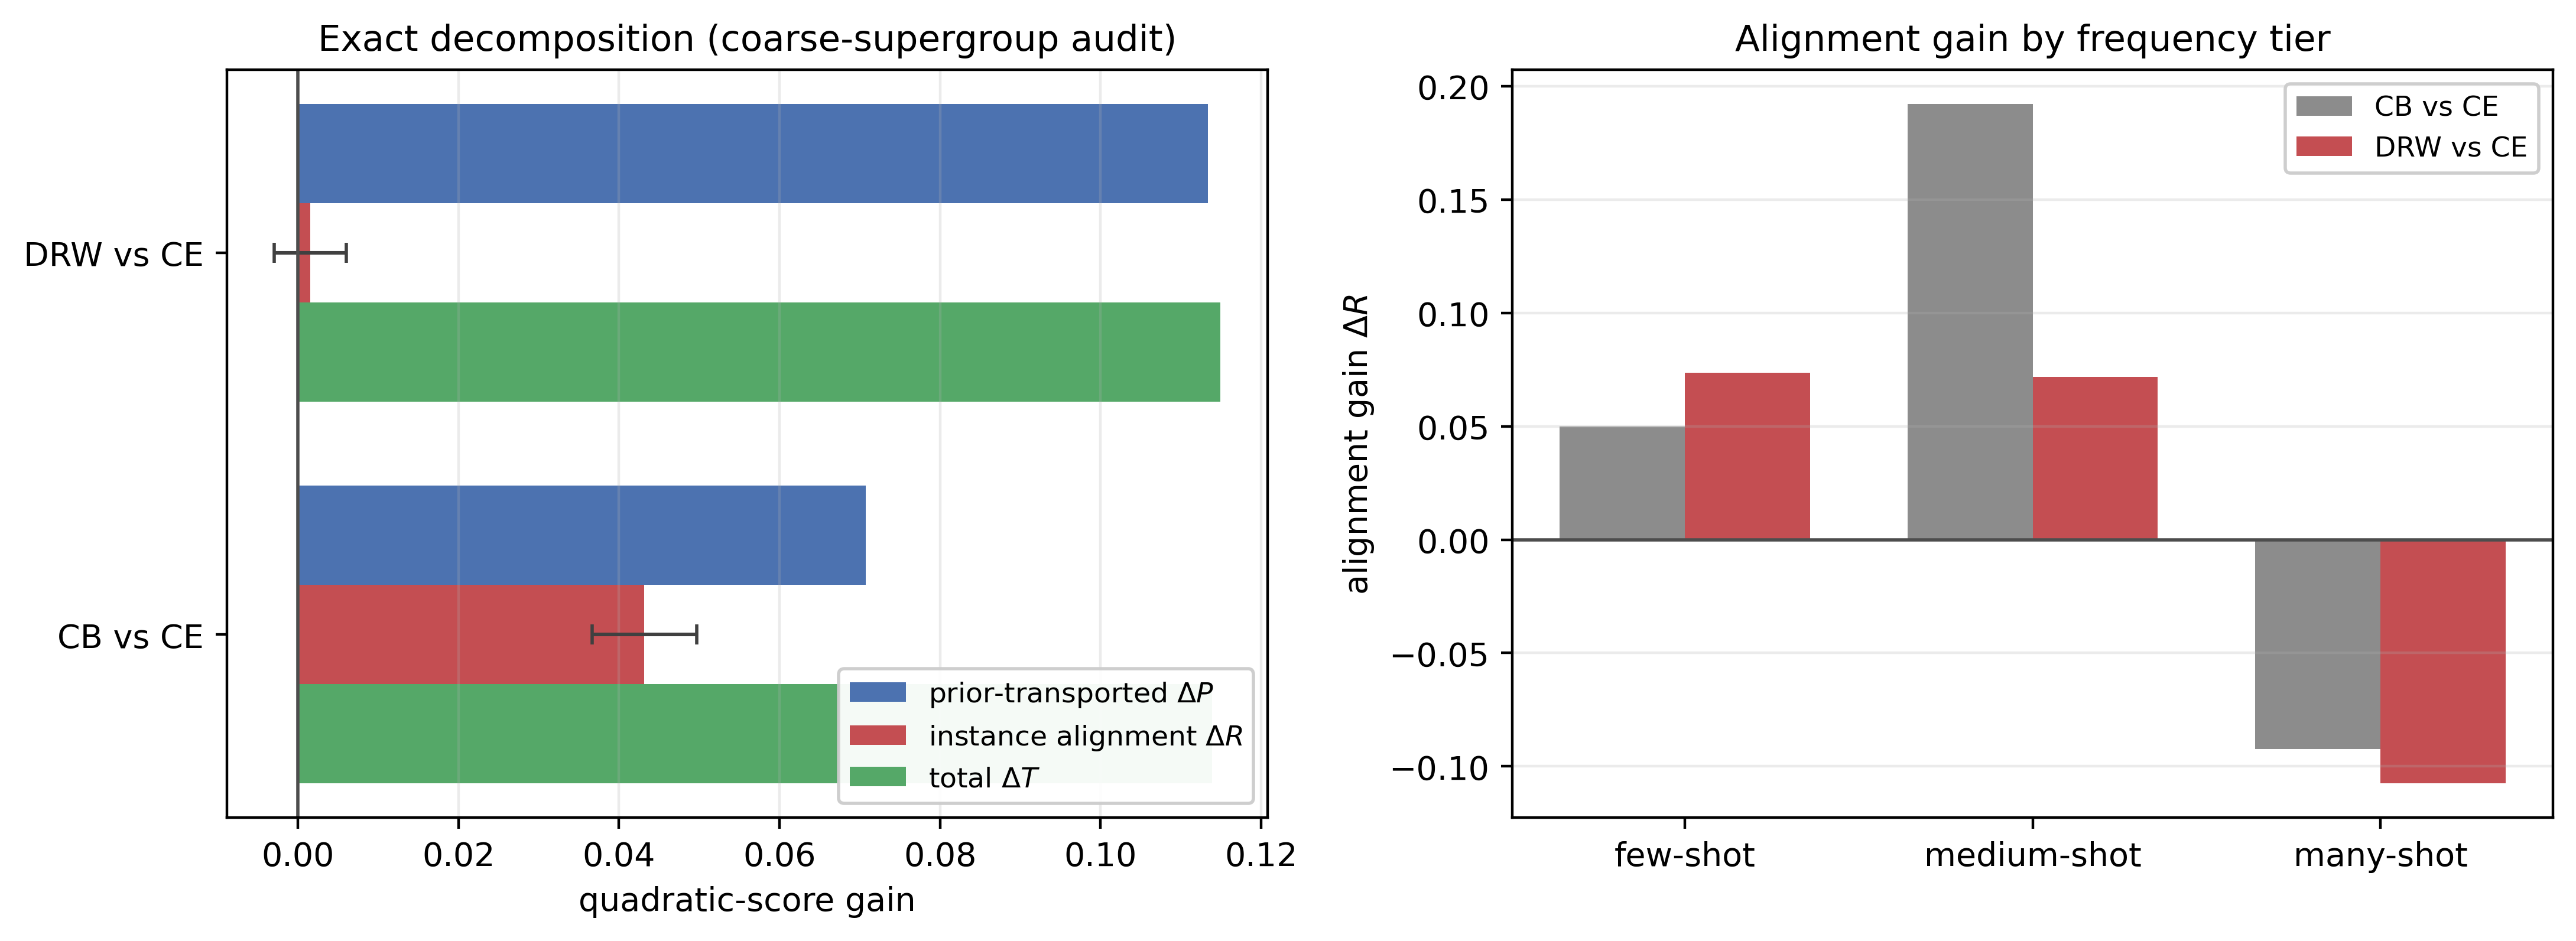
\includegraphics[width=\textwidth]{figures/fig8_text_lt.png}
\caption{\textbf{A third domain, with neither a spatial nor a class-frequency prior.}
Left: exact decomposition at the coarse-topic audit; CB's total gain is genuinely split
between both channels while DRW's is almost entirely transported. Error bars are
95\% H\'ajek intervals on $\widehat{\Delta R}$. Right: covariance gain by
training-frequency tier for both schedules, showing the same head-loses/tail-gains
signature as Figure~\ref{fig:cifar} despite the change of domain and grouping variable.}
\label{fig:textlt}
\end{figure*}

Table~\ref{tab:textlt-tier} breaks the superclass-audit covariance down by
training-frequency tier for both schedules; the two methods agree in shape even though
their superclass totals diverge sharply in composition, each gaining covariance on rare
and medium-frequency categories and losing it on frequent ones, the same qualitative
signature Section~\ref{app:lt} reports for image classification.

\begin{table}[t]
\centering
\caption{Covariance gain by training-frequency tier at the superclass audit,
20-Newsgroups-LT. Both schedules gain within-group covariance on rare and medium categories
and lose it on frequent ones.}
\label{tab:textlt-tier}
\begin{tabular}{@{}lrrr@{}}
\toprule
Tier & $n$ & $\widehat{\Delta R}$, CB vs CE & $\widehat{\Delta R}$, DRW vs CE \\
\midrule
Few-shot ($<20$)          & 1954 & $0.04991$  & $0.07352$  \\
Medium-shot ($20$--$100$) & 2610 & $0.19213$  & $0.07171$  \\
Many-shot ($>100$)        & 2968 & $-0.09227$ & $-0.10753$ \\
\bottomrule
\end{tabular}
\end{table}

This third domain uses a single trained pair per schedule rather than the multi-seed,
calibration-matched protocol Section~\ref{app:lt} applies to CIFAR-100-LT; extending
that fuller protocol to text is the natural next replication, not a step this section
claims to have taken.
